\documentclass{article}

\usepackage{geometry}
\usepackage{xeCJK}
\usepackage{amsmath}
\usepackage{tikz}
\usepackage{pgfplots}
% figure[H] float
\usepackage{float}
% subfigure
\usepackage{subcaption}
\usepackage{amssymb}
\usepackage{hyperref}
\usepackage{setspace}
% 字体底部样式:下划线、波浪线等
\usepackage{ulem}
% 修改公式编号
\usepackage{chngcntr}

% make cdot thicker,比 cdot 更粗的圆点
\makeatletter
\newcommand*\bigcdot{\mathpalette\bigcdot@{.5}}
\newcommand*\bigcdot@[2]{\mathbin{\vcenter{\hbox{\scalebox{#2}{$\m@th#1\bullet$}}}}}
\makeatother

% 设置行间距 1.5 倍
\renewcommand{\baselinestretch}{1.5}
% 自定义图片的标题:Figure -> 图
\renewcommand{\figurename}{图}
% 自定义表格的标题:Table -> 表
\renewcommand{\tablename}{表}

% 设置页大小和页边距,或者scale=0.8
\geometry{a4paper,left=3.18cm,right=3.18cm,top=2.54cm,bottom=2.54cm}
% 兼容
\pgfplotsset{compat=1.16}
% 中文默认没有斜体和粗体格式,开启伪斜体和指定黑体;
\setCJKmainfont[AutoFakeSlant, BoldFont=SimHei]{SimSun}
\usetikzlibrary{positioning}
% area of hatch,面积阴影部分
\usetikzlibrary{patterns}
% 箭头类型
\usetikzlibrary{arrows.meta}

\hypersetup{
    colorlinks,
    citecolor=black,
    filecolor=black,
    linkcolor=black,
    urlcolor=black
}
% 定义amsmath arccot, ch, sh
\DeclareMathOperator{\arccot}{arccot}
\DeclareMathOperator{\ch}{ch}
\DeclareMathOperator{\sh}{sh}
% 每个章节后,重置公式编号
\counterwithin*{equation}{section}

% 修改公式标签引用颜色
\def\eqref#1{{\color{blue}\hypersetup{linkcolor=blue} (\ref{#1}) }}
% 修改图片标签引用的颜色
\def\figureref#1{{\color{blue}\hypersetup{linkcolor=blue} (\ref{#1}) }}
% 修改跳转标签引用的颜色
\def\linkref[#1]#2{\hyperref[#1]{\color{blue}\ #2\ }}

% 添加 input 搜索目录
\makeatletter
\def\input@path{
  {../latex_package/}
  {./1_functions_and_limits/}
  {./2_derivative_and_integral/}
  {./3_mean_value_theorem_and_application/}
  {./4_indefinite_integrals/}
}
\makeatother

% 文字顶部和底部的弧度,使用自定义的包,避免输出错误字体文字和 warning 提示
\usepackage{./arcs/arcs}

\begin{document}
  \tableofcontents

  \newpage
  \part{函数与极限}
  \section{集合}
    \subsection{表示法}
\begin{enumerate}
  \item 列举法:$A = \{a_1, a_2, ..., a_n\}$
  \item 描述法:$M = \{x | \text{x具有性质P} \}$
\end{enumerate}

\subsection{数集}
\paragraph{}
在字母右上角标 “*”,表示排除 0 元素的数集;
\paragraph{}
在字母右上角标 “+”,表示排除 0 元素与负数的数集。
\paragraph{}
例子:自然数集 N 和整数集 Z

\begin{gather}
N^* = \{1, 2, ..., n, ...\} \\
Z^+ = \{1, 2, ..., n, ...\}
\end{gather}

\subsection{集合关系}
\paragraph{}
子集、真子集、相等、空集(是任何集合的子集)

\subsection{集合运算}
\paragraph{}
并、交、差(\textbackslash)
\paragraph{}
差运算;如果 I 是全集(基本集),也相当于求 A 的补集(余集):

\begin{equation}
I \backslash A = A^c = \{x | x \in I, x \notin A\}
\end{equation}

\paragraph{}
$A^c$ 是补集

\subsubsection{法则}
\begin{enumerate}
  \item 交换律:
    \begin{enumerate}
      \item $A \cup B = B \cup A$
      \item $A \cap B = B \cap A$
    \end{enumerate}
  \item 结合律:
    \begin{enumerate}
      \item $(A \cup B) \cup C = A \cup (B \cup C)$
      \item $(A \cap B) \cap C = A \cap (B \cap C)$
    \end{enumerate}
  \item 分配律:
    \begin{enumerate}
      \item $(A \cup B) \cap C = (A \cap C) \cup (B \cap C)$
      \item $(A \cap B) \cup C = (A \cup C) \cap (B \cup C)$
    \end{enumerate}
  \item 对偶律:
    \begin{enumerate}
      \item ${(A \cup B)}^c = A^c \cap B^c$
      \item ${(A \cap B)}^c = A^c \cup B^c$
    \end{enumerate}
\end{enumerate}

\subsubsection{直积}
\begin{equation}
A \times B = \{(x, y) | x \in A, y \in B\}
\end{equation}

\subsection{区间和邻域}

\subsubsection{区间}
\paragraph{}
(a, b)、[a, b]、[a, b)、(a, b]
\subsubsection{邻域}

\paragraph{}
邻域:
\begin{equation}
U(a, \delta) = \{x | a - \delta < x < a + \delta\}
\end{equation}

\paragraph{}
去心邻域:
\begin{equation}
\mathring{U}(a, \delta) = \{x | 0 < |x - a| < \delta\}
\end{equation}

  \section{映射}
    \begin{enumerate}
  \item 非空集合 $X, Y$
  \item 法则 $f$
  \item $X$ 中的每个元素 $x$,在法则 $f$ 下,能从 $Y$ 中找到\textbf{唯一}的值 $y$ ,即: $y = f(x)$
\end{enumerate}

\begin{equation}
f:X \to Y
\end{equation}

\paragraph{}
x与y关系:一对一、多对一


\begin{figure}[H]
\centering
  %------- 第1行 -------
  \begin{subfigure}[t]{0.4\linewidth}
    \centering
      % x 与 y 关系,一对一
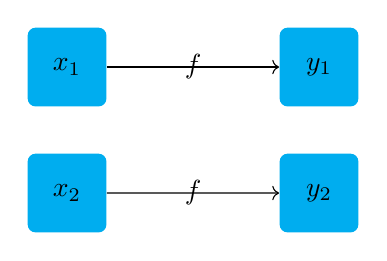
\begin{tikzpicture}[scale=0.8]
  \node [fill=cyan,minimum size=1cm,rounded corners=.1cm]   (x1) at (0,0)    {$x_1$};
  \node [fill=cyan,minimum size=1cm,rounded corners=.1cm]   (x2) at (0,-2)   {$x_2$};
  \node [fill=cyan,minimum size=1cm,rounded corners=.1cm]   (y1) at (4,0)   {$y_1$};
  \node [fill=cyan,minimum size=1cm,rounded corners=.1cm]   (y2) at (4,-2)   {$y_2$};

  \draw [->] (x1) -- (y1) node[midway] {$f$};
  \draw [->] (x2) -- (y2) node[midway] {$f$};
\end{tikzpicture}

      \caption{一对一}
  \end{subfigure}
  \begin{subfigure}[t]{0.4\linewidth}
    \centering
      % x 与 y 关系,多对一
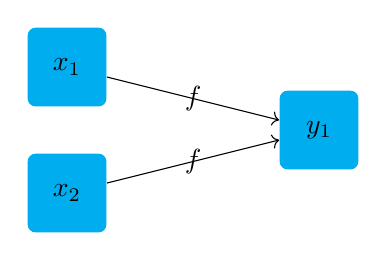
\begin{tikzpicture}[scale=0.8]
  \node [fill=cyan,minimum size=1cm,rounded corners=.1cm]   (x1) at (0,0)    {$x_1$};
  \node [fill=cyan,minimum size=1cm,rounded corners=.1cm]   (x2) at (0,-2)   {$x_2$};
  \node [fill=cyan,minimum size=1cm,rounded corners=.1cm]   (y1) at (4,-1)   {$y_1$};

  \draw [->] (x1) -- (y1) node[midway] {$f$};
  \draw [->] (x2) -- (y1) node[midway] {$f$};
\end{tikzpicture}

      \caption{多对一}
  \end{subfigure}
  \caption{x 与 y 关系}
\end{figure}

\paragraph{}
\textbf{概念}

\begin{enumerate}
  \item 定义域(Domain):$D_f = X$
  \item 值域(Range):$R_f = Y = f(x)$
\end{enumerate}

\begin{enumerate}
  \item 满射:$Y$ 中任意一个元素 $y$,都是 $X$ 中某一元素的像
  \item 单射:$X$ 中任意两个元素 $x_1 \neq  x_2$,它们的像不一样,$f(x_1) \neq  f(x_2)$
  \item 双射(一一映射):满足单射和满射条件
\end{enumerate}

\subsection{逆映射}

\begin{enumerate}
  \item $f$ 是 $X$ 到 $Y$ 的单射
  \item 则逆映射 $f^{-1} = g$,值域 $R_f$ 到 $X$ 的映射,即 $g(y) = x$
\end{enumerate}

\begin{equation}
g:R_f \to X
\end{equation}

\subsection{复合映射}

\begin{enumerate}
  \item 设有两个映射 $g:X \to Y_1$,$f:Y_2 \to Z$
  \item $Y_1 \subset Y_2$
  \item 则 $X$ 到 $Z$ 的映射,记作:$f \circ g$
\end{enumerate}

\begin{gather}
f \circ g: X \to Z \\
(f \circ g)(x) = f[g(x)], x \in X
\end{gather}

  \section{函数}
    \subsection{函数}
\paragraph{}
在数集上的映射,$D \subset R$,$f:D \to R$ 称为函数。

\subsection{函数的表示}

\begin{enumerate}
  \item 表格法
  \item 图形法
  \item  解析法(公式法)
\end{enumerate}

\subsection{函数的特性}

\subsubsection{有界性}

\begin{enumerate}
  \item 上界:存在数 $K_1$,满足 $\forall{x},\ f(x) \leq K_1$
  \item 下界:存在数 $K_2$,满足 $\forall{x},\ f(x) \geq K_2$
  \item 有界:存在正数 $M$,满足 $\forall{x},\ |f(x)| \leq M$
  \item 无界:不存在 $M$ 使得第 3 点的公式成立
\end{enumerate}

\subsubsection{单调性}
\paragraph{}
在区间上的单调性:设函数 $f(x)$ 的定义域为 $D$ ,在区间 $I \subset D$ 上的任意两点 $x_1, x_2$,且 $x_1 < x_2$,恒有:

\begin{enumerate}
  \item 单调增加:$f(x_1) < f(x_2)$
  \item 单调减少:$f(x_1) > f(x_2)$
\end{enumerate}

\subsubsection{奇偶性}
\paragraph{}
函数 $f(x)$ 的定义域 $D$ 关于原点对称,如果 $\forall x \in D$,满足:

\begin{enumerate}
  \item 偶函数:$f(-x) = f(x)$
  \item 奇函数:$f(-x) = -f(x)$
\end{enumerate}

\subsubsection{周期性}
\paragraph{}
设函数 $f(x)$ 的定义域为 $D$,存在正整数 $l$,使得任一 $x \in D$,有 $(x \pm l) \in D$,且
 $f(x + l) = f(x)$ 恒成立。

\subsection{反函数与复合函数}

\subsubsection{反函数}
\paragraph{}
设函数 $f:D \rightarrow f(D)$ 是单射,则它存在逆函数 $f^{-1}:f(D) \rightarrow D$,称此函数 $f^{-1}$ 为 $f$ 的反函数。

\subsubsection{复合函数}
\paragraph{}
设函数 $y = f(u)$ 的定义域为 $D_f$,函数 $u = g(x)$ 的定义域为 $D_g$ 且其值域 $R_g \subset D_f$,则由下式确定的函数:

\begin{equation}
y = f[g(x)], x \in D_g
\end{equation}

\paragraph{}
称为由函数 $u = g(x)$ 与函数 $y = f(u)$ 构成的复合函数,变量 $u$ 称为中间变量。

\subsection{函数的运算}
\paragraph{}
设函数 $f(x), g(x)$ 的定义域分别是 $D_1, D_2$,$D = D_1 \cap D_2 \neq \varnothing$,则可以定义下列运算:

\begin{enumerate}
  \item 和(差)$f \pm g$:$(f \pm g)(x) = f(x) \pm g(x), x \in D$
  \item 积$f \cdot g$:$(f \cdot g)(x) = f(x) \cdot g(x), x \in D$
  \item 商$\frac{f}{g}$:$(\frac{f}{g})(x) = \frac{f(x)}{g(x)}, x \in D  \backslash \{x|g(x) = 0, x \in D\}$
\end{enumerate}

\subsection{初等函数}

\begin{enumerate}
  \item 幂函数
  \item 指数函数
  \item 对数函数
  \item 三角函数
  \item 反三角函数
\end{enumerate}

\subsection{双曲函数}
\subsubsection{双曲正弦}
\paragraph{}
$sh \, x = \frac{e^x - e^{-x}}{2}$

\begin{figure}[H]
  \centering
    % sh(x) = (e^x - e^(-x)) / 2
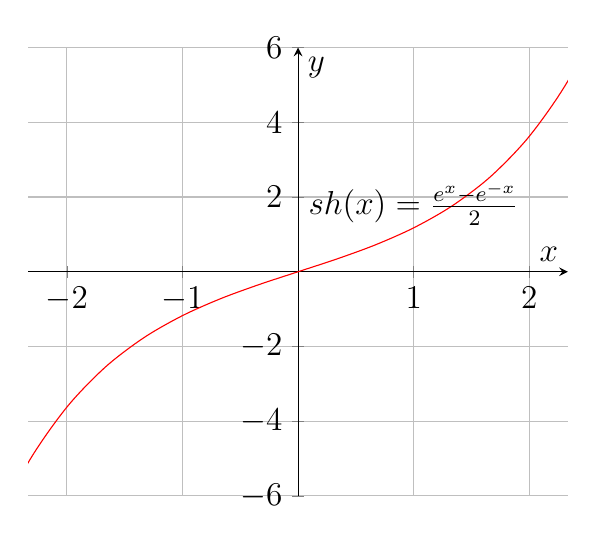
\begin{tikzpicture}
  \begin{axis}[domain=-4:4,ymin=-6,ymax=6, grid=both, font=\large, axis lines = middle, smooth, xlabel={$x$}, ylabel={$y$}]
    \addplot[draw=red] {(e^x - e^(-x)) / 2};
    \node at (axis cs:1,1.8) {$sh(x) = \frac{e^x - e^{-x}}{2}$};
  \end{axis}
\end{tikzpicture}

    \caption{$sh(x) = \frac{e^x - e^{-x}}{2}$}
    \label{sh_x}
\end{figure}

\subsubsection{双曲余弦}
\paragraph{}
$ch \, x = \frac{e^x + e^{-x}}{2}$

\begin{figure}[H]
  \centering
    % ch(x) = (e^x + e^(-x)) / 2
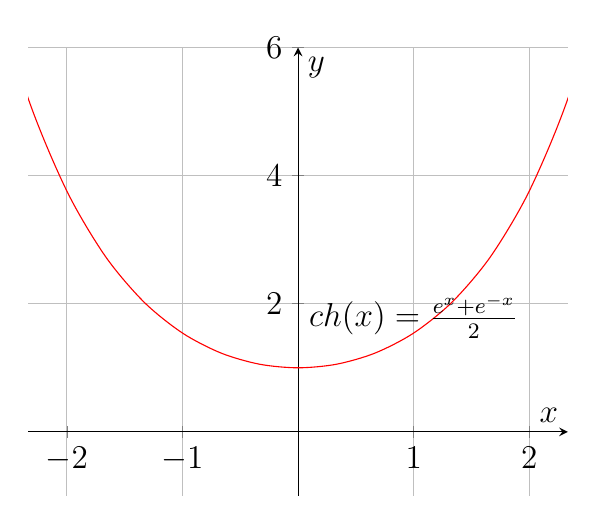
\begin{tikzpicture}
  \begin{axis}[domain=-4:4,ymin=-1,ymax=6, grid=both, font=\large, axis lines = middle, smooth, xlabel={$x$}, ylabel={$y$}]
    \addplot[draw=red] {(e^x + e^(-x)) / 2};
    \node at (axis cs:1,1.8) {$ch(x) = \frac{e^x + e^{-x}}{2}$};
  \end{axis}
\end{tikzpicture}

    \caption{$ch(x) = \frac{e^x + e^{-x}}{2}$}
    \label{ch_x}
\end{figure}

\subsubsection{双曲正切}
\paragraph{}
$th \, x = \frac{sh \, x}{ch \, x} = \frac{e^x - e^{-x}}{e^x + e^{-x}}$


\begin{figure}[H]
  \centering
    % th(x) = (e^x - e^(-x)) / (e^x -+e^(-x))
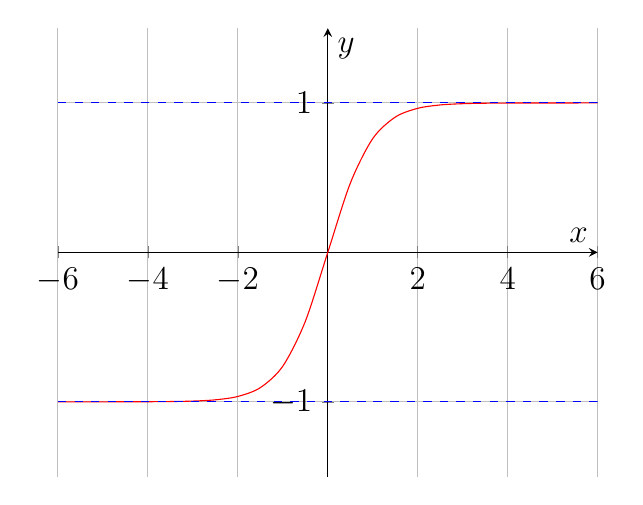
\begin{tikzpicture}
  \begin{axis}[domain=-6:6,ymin=-1.5,ymax=1.5, grid=both, font=\large, axis lines = middle, smooth, xlabel={$x$}, ylabel={$y$}]
    \addplot[draw=red] {(e^x - e^(-x)) / (e^x + e^(-x))};
    \addplot[dashed, draw=blue] {-1};
    \addplot[dashed, draw=blue] {1};
    \node at (axis cs:1,1.8) {$th(x) = \frac{e^x - e^{-x}}{e^x + e^{-x}}$};
  \end{axis}
\end{tikzpicture}

    \caption{$th(x) = \frac{e^x - e^{-x}}{e^x + e^{-x}}$}
    \label{th_x}
\end{figure}

\subsection{反双曲函数}
\subsubsection{反双曲正弦}
\paragraph{}
$y = arsh \, x = \ln(x + \sqrt{x^2 + 1})$

\begin{figure}[H]
  \centering
    % y = arsh(x)
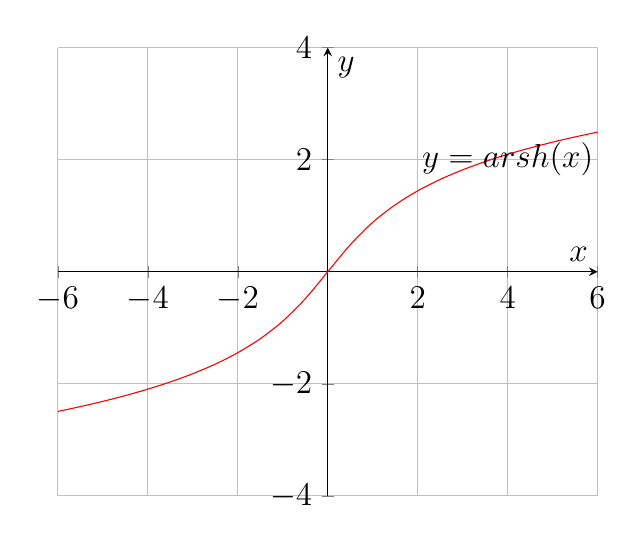
\begin{tikzpicture}
  \begin{axis}[domain=-6:6,ymin=-4,ymax=4, grid=both, font=\large, axis lines = middle, smooth, xlabel={$x$}, ylabel={$y$}]
    \addplot[draw=red] {ln(x + sqrt(x^2 + 1))};
    \node at (axis cs:4,2) {$y = arsh(x)$};
  \end{axis}
\end{tikzpicture}

    \caption{$y = arsh(x)$}
    \label{arsh_x}
\end{figure}

\subsubsection{反双曲余弦}
\paragraph{}
$y = arch \, x = \ln(x + \sqrt{x^2 - 1})$

\begin{figure}[H]
  \centering
    % y = arch(x)
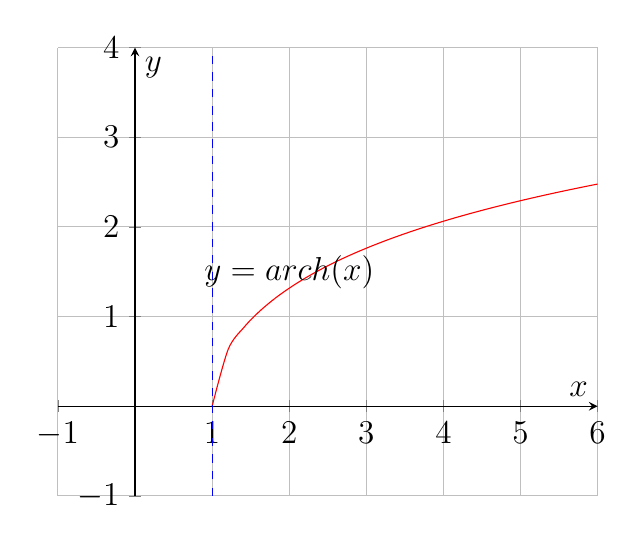
\begin{tikzpicture}
  \begin{axis}[xmin=-1, xmax=6,ymin=-1,ymax=4, grid=both, font=\large, axis lines = middle,
    smooth, xlabel={$x$}, ylabel={$y$}]
    \addplot[draw=red,domain=1:6] {ln(x + sqrt(x^2 - 1))};
    \addplot[dashed, draw=blue, mark=none] coordinates {(1, -1) (1, 4)};
    \node at (axis cs:2,1.5) {$y = arch(x)$};
  \end{axis}
\end{tikzpicture}

    \caption{$y = arch(x)$}
    \label{arch_x}
\end{figure}

\subsubsection{反双曲正切}
\paragraph{}
$y = arth \, x = \frac{1}{2} \ln(\frac{1 + x}{1 - x})$

\begin{figure}[H]
  \centering
    % y = arth(x)
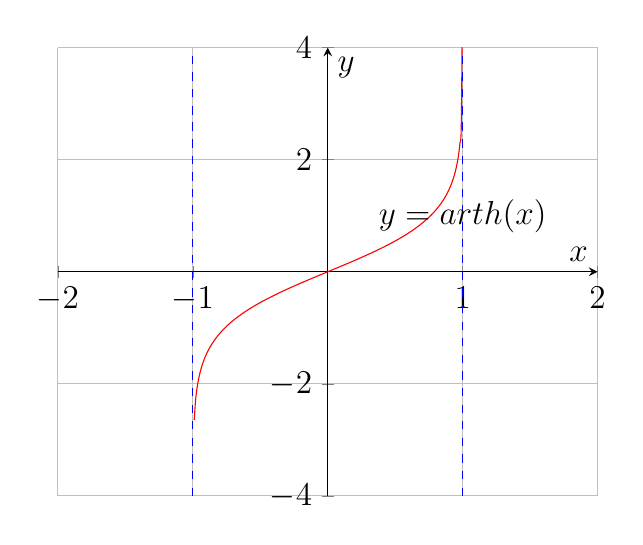
\begin{tikzpicture}
  \begin{axis}[xmin=-2,xmax=2,ymin=-4,ymax=4, grid=both, font=\large, axis lines=middle, smooth, xlabel={$x$}, ylabel={$y$}]
    \addplot[draw=red,domain=-1:1,samples=200] {(1/2)*ln((1 + x)/(1 - x))};
    \addplot[dashed, draw=blue, mark=none] coordinates {(1, -4) (1, 4)};
    \addplot[dashed, draw=blue, mark=none] coordinates {(-1, -4) (-1, 4)};
    \node at (axis cs:1,1) {$y = arth(x)$};
  \end{axis}
\end{tikzpicture}

    \caption{$y = arth(x)$}
    \label{arth_x}
\end{figure}

  \section{数列的极限}
    \subsection{数列}
\paragraph{}
如果按照某一法则,对每个$n \in N^+$,对应着一个确定的实数$x_n$,这些实数$x_n$按照下标$n$ 从小到大排序得到的一个序列,

\begin{equation}
x_1, x_2, x_3, ..., x_n, ...
\end{equation}

\paragraph{}
就叫数列,简记为数列 $\{x_n\}$。

\paragraph{}
$x_n$ 为一般项。

\subsection{数列极限}
\paragraph{}
设 $\{x_n\}$ 为一数列,如果存在常数 $a$,对于任意给定的正整数 $\varepsilon$(无论它多么小),总存在正整数 $N$ ,使得当 $n > N$ 时,不等式

\begin{equation}
|x_n - a| < \varepsilon,
\end{equation}

\paragraph{}
都成立,那么就称常数 $a$ 是数列 $\{x_n\}$ 的极限,或者称数列 $\{x_n\}$ 收敛于 $a$,记为

\begin{equation}
\lim_{n \to \infty} x_n = a,
\end{equation}

\paragraph{}
或

\begin{equation}
x_n \to a (n \to \infty).
\end{equation}

\paragraph{}
如果不存在这样的常数 $a$,就说数列 $\{x_n\}$ 是发散的。

\subsection{收敛数列的性质}
\subsubsection{极限的唯一性}
\paragraph{}
如果数列 $\{x_n\}$ 收敛,那么它的极限值唯一。

\subsubsection{收敛数列的有界性}
\paragraph{}
如果数列 $\{x_n\}$ 收敛,那么数列 $\{x_n\}$ 一定有界。

\subsubsection{收敛数列的保号性}
\paragraph{}
如果 $\displaystyle{\lim_{n \to \infty}} x_n = a$,且 $a > 0$(或 $a < 0$),那么存在正整数 $N > 0$,当 $n > N$ 时,都有 $x_n > 0$(或 $x_n < 0$)。

\subsubsection{收敛数列与其子数列间的关系}
\paragraph{}
如果数列 $\{x_n\}$ 收敛于 $a$,那么它的任一子数列也收敛,且极限也是 $a$。

  \section{函数的极限}
    \subsection{自变量趋于有限值时函数的极限}
\paragraph{}
设函数 $f(x)$ 在点 $x_0$ 的某一去心邻域内有定义,如果存在常数 $A$,对于任意给定的正数 $\varepsilon$(无论它多么小),总存在正数 $\delta$,使得当 $x$ 满足不等式 $0 < |x - x_0| < \delta$ 时,对应的函数值 $f(x)$ 都满足不等式

\begin{equation}
|f(x) - A| < \varepsilon,
\end{equation}

\paragraph{}
那么常数 $A$ 就叫做函数 $f(x)$ 当 $x \to x_0$ 时的极限,记作

\begin{equation}
\lim_{x \to x_0} f(x) = A,
\end{equation}

\paragraph{}
或

\begin{equation}
f(x) \to A(\text{当~~} x \to x_0).
\end{equation}

\subsubsection{单侧极限}
\paragraph{}
从 $x_0$ 的左侧或右侧趋近,即 $x_0 - \delta < x < x_0$ 或 $x_0 < x < x_0 + \delta$:

\begin{enumerate}
  \item 左极限:$\displaystyle{\lim_{x \to {x_0}^-}} f(x) = A \text{~~或~~} f({x_0}^-) = A$
  \item 右极限:$\displaystyle{\lim_{x \to {x_0}^+}} f(x) = A \text{~~或~~} f({x_0}^+) = A$
\end{enumerate}

\subsection{自变量趋于无穷大时函数的极限}
\paragraph{}
设函数 $f(x)$ 当 $|x|$ 大于某一正数时有定义,如果存在常数 $A$,对于任意给定的正整数 $\varepsilon$(无论它多么小),总存在着正数 $X$,使得当 $x$ 满足不等式 $|x| > X$ 时,对应的函数值 $f(x)$ 都满足不等式

\begin{equation}
|f(x) - A| < \varepsilon,
\end{equation}

\paragraph{}
那么常数 $A$ 就叫做函数 $f(x)$ 当 $x \to \infty$ 时的极限,记作

\begin{equation}
\lim_{x \to \infty} f(x) = A \text{~~或~~} f(x) \to A (\text{当~~} x \to \infty).
\end{equation}

\subsection{函数极限的性质}
\paragraph{}
下面的性质仅以 $\displaystyle{\lim_{x \to x_0}}f(x)$ 形式为代表给出的性质。

\subsubsection{函数极限的唯一性}
\paragraph{}
如果 $\displaystyle{\lim_{x \to x_0}}f(x)$ 存在,那么这极限唯一。

\subsubsection{函数极限的局部有界性}
\paragraph{}
如果 $\displaystyle{\lim_{x \to x_0}}f(x) = A$,那么存在常数 $M > 0$ 和 $\delta > 0$,使得当 $0 < |x - x_0| < \delta$ 时,有 $|f(x)| \leq M$.

\subsubsection{函数极限的局部保号性}
\paragraph{}
如果 $\displaystyle{\lim_{x \to x_0}}f(x) = A$,且 $A > 0 (\text{或~~} A < 0)$,那么存在常数 $\delta > 0$,使得当 $0 < |x - x_0| < \delta$ 时,有 $f(x) > 0 (\text{或~~} f(x) < 0)$。

\subsubsection{函数极限与数列极限的关系}
\paragraph{}
如果极限 $\displaystyle{\lim_{x \to x_0}}f(x)$ 存在,$\{x_n\}$ 为函数 $f(x)$ 的定义域内任一收敛于 $x_0$ 的数列,且满足 $x_n \neq x_0(n \in N^+)$,那么相应的函数值数列 $\{f(x_n)\}$ 必收敛,且 $\displaystyle{\lim_{n \to \infty}f(x_n) = \lim_{x \to x_0}f(x)}$。

  \section{无穷小与无穷大}
    \subsection{无穷小}
\paragraph{}
如果函数 $f(x)$ 当 $x \to x_0(\text{或~~} x \to \infty)$ 时的极限为零,那么称函数 $f(x)$ 为当 $x \to x_0(\text{或~~} x \to \infty)$ 时的无穷小。

\paragraph{}
无穷小与函数极限的关系:

\paragraph{}
\textbf{定理1} 在自变量的同一变化过程 $x \to x_0(\text{或~~} x \to \infty)$ 中,函数 $f(x)$ 具有极限 $A$ 的充分必要条件是 $f(x) = A + a$,其中 $a$ 是无穷小.

\subsection{无穷大}
\paragraph{}
设函数 $f(x )$ 在 $x_0$ 的某一去心邻域内有定义(或 $|x|$ 大于某一正数时有定义),如果对于任意给定的正数 $M$(无论它多么大),总存在正数 $\delta$(或正数 $X$),只要 $x$ 适合不等式 $0 < |x - x_0| < \delta (\text{或} |x| > X)$,对应的函数值 $f(x)$ 总满足不等式

\begin{equation}
|f(x)| > M,
\end{equation}

\paragraph{}
则称函数 $f(x)$ 为当 $x \to x_0(\text{或} x \to \infty)$ 时的无穷大,记作

\begin{gather}
\lim_{x \to x_0}f(x) = \infty \\
(\text{或} \lim_{x \to \infty}f(x) = \infty).
\end{gather}

\paragraph{}
正无穷大和负无穷大:

\begin{gather}
f(x) > M, \lim_{x \to x_0 (\text{或}x \to \infty)} f(x) = + \infty; \\
f(x) < - M, \lim_{x \to x_0 (\text{或}x \to \infty)} f(x) = - \infty.
\end{gather}

\paragraph{}
\textbf{定理2} 在自变量的同一变化过程中,如果 $f(x)$ 为无穷大,则 $\frac{1}{f(x)}$ 为无穷小;反之,如果 $f(x)$ 为无穷小,且 $f(x) \neq 0$,则 $\frac{1}{f(x)}$ 为无穷大.

  \section{极限运算法则}
    \subsection{定理}
\paragraph{}
以下结论适合 $x \to x_0 (\text{或} x \to \infty)$。

\subsubsection{定理1}
\paragraph{}
有限个无穷小的和也是无穷小。

\subsubsection{定理2}
\paragraph{}
有界函数与无穷小的乘积是无穷小。

\paragraph{}
\textbf{推论1} 常数与无穷小的乘积是无穷小。

\paragraph{}
\textbf{推论2} 有限个无穷小的乘积是无穷小.

\subsubsection{定理3}
\paragraph{}
如果 $\lim f(x) = A, \lim g(x) =B$,那么

\begin{enumerate}
  \item $\lim [f(x) \pm g(x)] = \lim f(x) \pm \lim g(x) = A \pm B$
  \item $\lim [f(x) \cdot g(x)] = \lim f(x) \cdot \lim g(x) = A \cdot B$
  \item 若 $B \neq 0$,则$\lim \frac{f(x)}{g(x)} = \frac{\lim f(x)}{\lim g(x)} = \frac{A}{B}$
\end{enumerate}

\paragraph{}
\textbf{推论1} 如果 $\lim f(x)$ 存在,而 $c$ 为常数,则 $\lim[cf(x)] = c \lim f(x)$。

\paragraph{}
\textbf{推论2} 如果 $\lim f(x)$ 存在,而 $n$ 是正整数,则 $\lim{[f(x)]}^n={[\lim f(x)]}^n$。

\subsubsection{定理4}
\paragraph{}
设有数列 $\{x_n\}$ 和 $\{y_n\}$,如果

\begin{equation}
\lim_{n \to \infty} x_n = A, \quad \lim_{n \to \infty} y_n = B
\end{equation}

\paragraph{}
那么

\begin{enumerate}
  \item $\displaystyle{\lim_{n \to \infty}(x_n \pm y_n) = A \pm B}$
  \item $\displaystyle{\lim_{n \to \infty}(x_n \cdot y_n) = A \cdot B}$
  \item 当 $y_n \neq 0 (n = 1, 2, ...)$ 且 $B \neq 0$ 时,$\displaystyle{\lim_{n \to \infty} \frac{x_n}{y_n}=\frac{A}{B}}$
\end{enumerate}

\subsubsection{定理5}
\paragraph{}
如果 $\varphi (x) \geq \psi (x)$,而 $\lim \varphi (x) = a, \lim \psi (x) = b$,那么 $a \geq b$。

\subsubsection{定理6 复合函数的极限运算法则}
\paragraph{}
设函数 $y = f[g(x)]$ 是由函数 $u = g(x)$ 与函数 $y = f(u)$ 复合而成,$f[g(x)]$ 在点 $x_0$ 的某去心邻域内有定义,若 $\displaystyle{\lim_{x \to x_0}g(x) = u_0, \lim_{u \to u_0} f(u) = A}$,且存在 $\delta_0 > 0$,当 $x \in \mathring{U}(x_0, \delta_0)$ 时,有 $g(x) \neq u_0$,则

\begin{equation}
\lim_{x \to x_0} f[g(x)] = \lim_{u \to u_0} f(u) = A  
\end{equation}

  \section{极限存在准则}
    \subsection{夹逼准则}
\paragraph{}
\textbf{准则1} 如果数列 $\{x_n\}$、$\{y_n\}$ 及 $\{z_n\}$ 满足下列条件:

\begin{enumerate}
  \item 从某项起,即 $\exists n_0 \in N$,当 $n > n_0$ 时,有 $y_n \leq x_n \leq z_n$
  \item $\displaystyle{\lim_{n \to \infty} y_n = a, \lim_{n \to \infty} z_n = a}$
\end{enumerate}

\paragraph{}
那么数列 $\{x_n\}$ 的极限存在,且 $\displaystyle{\lim_{n \to \infty} x_n = a}$。

\paragraph{}
\textbf{准则1} 如果

\begin{enumerate}
  \item 当 $x \in \mathring{U}(x_0, r)(\text{or~~}|x| > M)$ 时,$g(x) \leq f(x) \leq h(x)$
  \item $\displaystyle{\lim_{x \to x_0 (x \to \infty)} g(x) = A, \lim_{x \to x_0 (x \to \infty)} h(x) = A}$
\end{enumerate}

\paragraph{}
那么 $\displaystyle{\lim_{x \to x_0 (x \to \infty)} f(x)}$ 存在,且等于 $A$。

\subsection{单调有界数列必有极限}

\subsection{柯西极限存在准则}
\paragraph{}
数列 $\{x_n\}$ 收敛的充分必要条件是:对于任意给定的正数 $\varepsilon$,存在着这样的正整数 $N$,使得当 $m > N, n > N$ 时,就有 $|x_n - x_m| < \varepsilon$。

  \section{无穷小的比较}
    \paragraph{}
下面的 $\alpha$ 和 $\beta$ 都是同一个变量变化的过程的无穷小

\paragraph{}
如果 $\lim \frac{\beta}{\alpha} = 0$,就说 $\beta$ 是比 $\alpha$ 高阶的无穷小,记作 $\beta = o(\alpha)$;

\paragraph{}
如果 $\lim \frac{\beta}{\alpha} = \infty$,就说 $\beta$ 是比 $\alpha$ 低阶的无穷小;

\paragraph{}
如果 $\lim \frac{\beta}{\alpha} = c \neq 0$,就说 $\beta$ 与 $\alpha$ 是同阶无穷小;

\paragraph{}
如果 $\lim \frac{\beta}{\alpha^k} = c \neq 0, k > 0$,就说 $\beta$ 是关于 $\alpha$ 的 $k$ 阶无穷小;

\paragraph{}
如果 $\lim \frac{\beta}{\alpha} = 1$,就说 $\beta$ 与 $\alpha$ 是等价无穷小,记作 $\alpha \sim \beta$。

\paragraph{}
\textbf{定理1} $\beta$ 与 $\alpha$ 是等价无穷小的充分必要条件是 $\beta = \alpha + o(\alpha)$。

\paragraph{}
\textbf{定理2} 设 $\alpha \sim \alpha^\prime, \beta \sim \beta^\prime$,且 $\lim \frac{\beta^\prime}{\alpha^\prime}$ 存在,则 $\lim \frac{\beta}{\alpha} = lim \frac{\beta^\prime}{\alpha^\prime}$。

  \section{函数的连续性和间断点}
    \subsection{连续性}
\subsubsection{增量}
\paragraph{}
设变量 $u$ 从它的一个初值 $u_1$ 变到终值 $u_2$,终值与初值的差 $u_2 - u_1$ 就叫做变量 $u$ 的增量,记作 $\Delta u$,即

\begin{equation}
\Delta u = u_2 - u_1
\end{equation}

\paragraph{}
增量可以正,也可以负

\paragraph{}
$x$ 从 $x_0$ 变到 $x_0 + \Delta x$ 时,函数 $y$ 相应的从 $f(x_0)$ 变到 $f(x_0 + \Delta x)$,因此函数 $y$ 的增量为:

\begin{equation}
\Delta y = f(x_0 + \Delta x) - f(x_0)
\end{equation}

\subsubsection{连续性定义}
\paragraph{}
\textbf{定义:}设函数 $y = f(x)$ 在点 $x_0$ 的某一邻域内有定义,如果
\begin{gather}
\lim_{\Delta x \to 0}\Delta y = \lim_{\Delta x \to 0}[f(x_0 + \Delta x) - f(x_0)] = 0, \\
\text{或} \lim_{x \to x_0} f(x) = f(x_0).
\end{gather}

\paragraph{}
那么就称函数 $y = f(x)$ 在点 $x_0$ 连续。

\paragraph{}
\textbf{左连续:}如果 $\lim_{x \to x_0^-} f(x) = f(x_0^-)$ 存在且等于 $f(x_0)$,即

\begin{equation}
f(x_0^-) = f(x_0)
\end{equation}

\paragraph{}
\textbf{右连续:}如果 $\lim_{x \to x_0^+}f(x) = f(x_0^+)$ 存在且等于 $f(x_0)$,即

\begin{equation}
f(x_0^+) = f(x_0)
\end{equation}

\paragraph{}
在区间上每一点都连续的函数,叫做函数在该区间上连续。

\subsection{间断点}
\paragraph{}
设函数 $f(x)$ 在点 $x_0$ 的某去心邻域内有定义。在此前提,如果函数 $f(x)$ 有下列三种情形之一:

\begin{enumerate}
  \item 在 $x = x_0$ 没有定义
  \item 虽在 $x = x_0$ 有定义,但 $\lim_{x \to x_0}f(x)$ 不存在
  \item 前 2 点都成立,但 $\lim_{x \to x_0}f(x) \neq f(x_0)$
\end{enumerate}

\paragraph{}
则函数 $f(x)$ 在点 $x_0$ 为不连续,而点 $x_0$ 称为函数 $f(x)$ 的间断点。

  \section{连续函数的运算和初等函数的连续性}
    \subsection{连续函数的和、差、积、商的连续性}
\paragraph{}
\textbf{定理1:}设函数 $f(x)$ 和 $g(x)$ 在点 $x_0$ 连续,则它们的和(差)$f\pm g$ 、积 $f\cdot g$ 及商 $\frac{f}{g}(\text{当} g(x_0) \neq 0 \text{时})$ 都在点 $x_0$ 连续。

\subsection{反函数与复合函数的连续性}
\paragraph{}
\textbf{定理2:}如果函数 $y = f(x)$ 在区间 $I_x$ 上单调增加(或单调减少)且连续,那么它的反函数 $x = f^{-1}(y)$ 也对应的在区间 $I_y = \{y | y = f(x), x \in I_x\}$ 上单调增加(或单调减少)且连续。

\paragraph{}
\textbf{定理3:}设函数 $y = f[g(x)]$ 由函数 $u = g(x)$ 与函数 $y = f(u)$ 复合而成,$\mathring{U}(x_0) \subset D_{f \circ g}$,若 $\lim_{x \to x_0} g(x) = u_0$,而函数 $y = f(u)$ 在 $u = u_0$ 连续,则

\begin{equation}
\lim_{x \to x_0} f[g(x)] = \lim_{u \to u_0} f(u) = f(u_0).
\end{equation}

\paragraph{}
\textbf{定理4:}设函数 $y = f[g(x)]$ 是由函数 $u = g(x)$ 与函数 $y = f(u)$ 复合而成,$U(x_0) \subset D_{f \circ g}$,若函数 $u = g(x)$ 在 $x = x_0$ 连续,且 $g(x_0) = u_0$,而函数 $y = f(u)$ 在 $u = u_0$ 连续,则复合函数 $y = f[g(x)]$ 在 $x = x_0$ 也连续。

\subsection{初等函数的连续性}
\paragraph{}
初等函数在其定义域中都连续。

  \section{闭区间上连续函数的性质}
    \subsection{有界性与最大值最小值定理}
\paragraph{}
对于在区间 $I$ 上有定义的函数 $f(x)$,如果有 $x_0 \in I$,使得对于任一 $x \in I$ 都有

\begin{equation}
f(x) \leq f(x_0) (f(x) \geq f(x_0)),
\end{equation}

\paragraph{}
则称 $f(x_0)$ 是函数 $f(x)$ 在区间 $I$ 上的\textbf{最大值}(\textbf{最小值})。

\paragraph{}
\textbf{有界性与最大值最小值定理\;} 在闭区间上连续的函数在该区间上有界且一定能取得它的最大值和最小值。

\subsection{零点定理与介值定理}
\paragraph{}
\textbf{零点定理\;} 设函数 $f(x)$ 在闭区间 $[a,b]$ 上连续,且 $f(a)$ 与 $f(b)$ 异号(即 $f(a) \cdot f(b) < 0$),那么在开区间 $(a,b)$ 内至少有一点 $\xi$,使

\begin{equation}
f(\xi) = 0.
\end{equation}

\paragraph{}
\textbf{介值定理\;} 设函数 $f(x)$ 在闭区间 $[a,b]$ 上连续,且在这区间的端点取不同的函数值 $f(a) = A$ 及 $f(b) = B$,那么,对于 $A$ 与 $B$ 之间的任意一个数 $C$,在开区间 $(a,b)$ 内至少有一点 $\xi$,使得

\begin{equation}
f(\xi) = C (a < \xi < b).
\end{equation}

\paragraph{}
\textbf{推论\;} 在闭区间上连续的函数必取得介于最大值 $M$ 与最小值 $m$ 之间的任何值。

\subsection{一致连续性}
\paragraph{}
\textbf{定义\;} 设函数 $f(x)$ 在区间 $I$ 上有定义。如果对于任意给定的正数 $\varepsilon$,总存在着正数 $\delta$,使得对于区间 $I$ 上的任意两点 $x_1, x_2$,当 $|x_1 - x_2| < \delta$ 时,就有

\begin{equation}
|f(x_1) - f(x_2)| < \varepsilon,
\end{equation}

\paragraph{}
那么称函数 $f(x)$ 在区间 $I$ 上是一致性连续的。

\paragraph{}
\textbf{一致连续性定理\;} 如果函数 $f(x)$ 在闭区间 $[a,b]$ 上连续,那么它在该区间上一致连续。


  \newpage
  \part{导数与微分}
  \section{导数概念}
    \subsection{导数的引例}
\begin{enumerate}
  \item 速度问题:直线运动的速度
  \item 切线问题:曲线的切线
\end{enumerate}

\subsection{导数的定义}
\subsubsection{函数在一点处的导数与导函数}
\paragraph{}
\textbf{定义~~}设函数 $y = f(x)$ 在点 $x_0$ 的某个邻域内有定义,当自变量 $x$ 在 $x_0$ 处取得增量 $\Delta x$(点 $x_0 + \Delta x$ 仍在该邻域内)时,相应的函数取得增量 $\Delta y = f(x_0 + \Delta x) - f(x_0)$;如果 $\Delta y$ 与 $\Delta x$ 之比当 $\Delta x \to 0$ 时的极限存在,则称函数 $y = f(x)$ 在点 $x_0$ 处\textbf{可导},并称这个极限为函数 $y = f(x)$ 在点 $x_0$ 处的\textbf{导数},记为 $f'(x_0)$,即

\begin{equation}
f'(x_0) = \lim_{\Delta x \to 0} \frac{\Delta y}{\Delta x} = \lim_{\Delta x \to 0} \frac{f(x_0 + \Delta x) - f(x_0)}{\Delta x},
\end{equation}

\paragraph{}
也可记作 $y'|_{x = x_0}, \frac{dy}{dx}|_{x = x_0}$ 或 $\frac{df(x)}{dx}|_{x=x_0}$。

\paragraph{}
也可取不同的形式,常见的有:

\begin{gather}
f'(x_0) = \lim_{h \to 0} \frac{f(x_0 + h) - f(x_0)}{h} , \\
\text{和} \\
f'(x_0) = \lim_{x \to x_0}\frac{f(x) - f(x_0)}{x - x_0}
\end{gather}

\paragraph{}
极限不存在,就说函数 $y = f(x)$ 在点 $x_0$ 处不可导。由于 $\Delta x \to 0$ 时,比式 $\frac{\Delta y}{\Delta x} \to \infty$,函数 $y = f(x)$ 在点 $x_0$ 处导数无穷大。

\paragraph{}
如果函数 $y = f(x)$ 在开区间 $I$ 内的每点处都可导,就称函数 $f(x)$ 在开区间 $I$ 内可导,这就构成了一个新的函数,叫做原来函数 $y = f(x)$ 的导函数,记作 $y', f'(x), \frac{dy}{dx}$ 或 $\frac{df(x)}{dx}$。

\paragraph{}
把 $x_0$ 换成 $x$,即得导函数的定义式:

\begin{gather}
y' = \lim_{x \to 0}\frac{f(x + \Delta x) - f(x)}{\Delta x} , \\
\text{或} \\
f'(x) = \lim_{h \to 0} \frac{f(x + h) - f(x)}{h}.
\end{gather}

\paragraph{}
导函数 $f'(x)$ 简称导数,而 $f'(x_0)$ 是 $f(x)$ 在 $x_0$ 处的导数

\subsubsection{常见函数的导数公式}

\begin{align}
C' &= 0 \qquad \text{(C 为常数)} \\
(x^a)' &= ax^{a-1} \qquad \text{$(a \in Q)$} \\
(\sin x)' &= \cos x \\
(\cos x)' &= - \sin x \\
(e^x)' &= e^x \\
(a^x)' &= a^x \ln a \\
(\ln x)' &= \frac{1}{x} \\
(\log_a x)' &= \frac{1}{x}\log_a e
\end{align}

\subsubsection{单侧导数}
\paragraph{}
极限存在的充分必要条件是左、右极限都\textbf{存在且相等}:

\begin{gather}
\lim_{h \to 0^-}\frac{f(x_0 + h) - f(x_0)}{h} \qquad \text{(左导数)} \\
\lim_{h \to 0^+}\frac{f(x_0 + h) - f(x_0)}{h} \qquad \text{(右导数)}
\end{gather}

\subsection{导数的几何意义}
\paragraph{}
函数 $y = f(x)$ 在点 $x_0$ 处的导数 $f'(x_0)$ 在几何上表示曲线 $y = f'(x)$ 在点 $M(x_0, f(x_0))$ 处的切线的斜率,即:

\begin{equation}
f'(x_0) = \tan \alpha ,
\end{equation}

\paragraph{}
其中 $\alpha$ 是切线的倾角。

\begin{figure}[H]
  \centering
    % 导数的几何意义
\begin{tikzpicture}
  \begin{axis}[xmin=0, xmax=3,ymin=0,ymax=3, grid=none,
    xtick=\empty,ytick=\empty, font=\large, axis lines=middle,
    smooth, xlabel={$x$}, ylabel={$y$}]

    % 曲线
    \addplot[draw=red,domain=0.3:2.5] {(x - 1)^2 + 0.5};
    \node [above] at (axis cs:2,2.5) {$y = f(x_0)$};
    \draw[fill] (1.5,0.75) circle [radius=0.02];
    % 切线
    \addplot[draw=blue,domain=0.3:2.2] {x - 0.75};
    \node [right] at (axis cs:2.2,1.45) {$T$};

    % 辅助线和点
    \addplot[dashed, draw=cyan, mark=none] coordinates {(1.5, 0) (1.5, 0.75)};
    \node [above] at (axis cs:1.5,0.75) {$M$};

    % 倾角
    \draw (1,0) arc (0:45:0.25);
    \node [right] at (axis cs:1,0.1) {$\alpha$};
  \end{axis}
  % 原点
  \node [below left] at (0,0) {$O$};
  \node [below] at (3.45,0) {$x_0$};
\end{tikzpicture}

    \caption{几何意义}
    \label{derivative_geometric_meaning}
\end{figure}

\paragraph{}
过点 $M(x_0, y_0)$ 和切线斜率 $f'(x_0)$,根据直线的点斜式,得到\textbf{切线方程}:

\begin{equation}
y - y_0 = f'(x_0)(x - x_0)
\end{equation}

\paragraph{}
过点 $M(x_0, y_0)$ 和法线斜率 $-\frac{1}{f'(x_0)}, f'(x_0) \neq 0$,根据直线的点斜式,得到\textbf{法线方程}:

\begin{equation}
y - y_0 = - \frac{1}{f'(x_0)}(x - x_0), \; f'(x_0) \neq 0
\end{equation}

\subsection{函数可导性与连续性的关系}
\paragraph{}
设函数 $y = f(x)$ 在点 $x$ 处可导,即

\begin{equation}
\lim_{\Delta x \to 0} \frac{\Delta y}{\Delta x} = f'(x)
\end{equation}

\paragraph{}
存在。由具有极限的函数与无穷小的关系知道,

\begin{equation}
\frac{\Delta y}{\Delta x} = f'(x) + \alpha ,
\end{equation}

\paragraph{}
其中 $\alpha$ 为当 $\Delta x \to 0$ 时的无穷小。上式两边同乘以 $\Delta x$,得

\begin{equation}
\Delta y = f'(x) \Delta x + \alpha\Delta x.
\end{equation}

\paragraph{}
由此可见,当 $\Delta x \to 0$ 时,$\Delta y \to 0$。这就是说,函数 $y = f(x)$ 在点 $x$ 处是连续的。

\paragraph{}
所以,如果函数 $y = f(x)$ 在点 $x$ 处可导,则函数在该点必连续。

\paragraph{}
函数在某点的连续是函数在该点可导的必要条件,但不是充分条件(\textbf{可导即连续,但连续不一定可导})。

\paragraph{}
充分条件:条件 A $\to$ 结论 B,A 则为 B 充分条件

\paragraph{}
必要条件:结论 B $\to$ 条件 A,A 则为 B 必要条件

  \section{函数的求导法则}
    \subsection{函数的和、差、积、商的求导法则}
\paragraph{}
\textbf{定理1~~}如果函数 $u = u(x)$ 及  $v = v(x)$ 都在点 $x$ 具有导数,那么它们的和、差、积、商(除分母为零的点外)都在点 $x$ 具有导数,且

\begin{align}
\left[u(x) \pm  v(x)\right]' &= u'(x) \pm v'(x); \\
\left[u(x)v(x)\right]' &= u'(x)v(x) + u(x)v'(x); \\
\left[\frac{u(x)}{v(x)}\right]' &= \frac{u'(x)v(x) - u(x)v'(x)}{v^2(x)} \; (v(x) \neq 0).
\end{align}

\paragraph{}
定理 1 中的法则(1)、(2)可推广到任意有限个可导函数的情形,即

\begin{align}
(u + v - w)' &= u' + v' - w'; \\
(uvw)' &= u'vw + uv'w + uvw'; \\
(Cu)' &= Cu' \text{~~(C 为常数)}.
\end{align}

\subsection{反函数的求导法则}
\paragraph{}
\textbf{定理2~~}如果函数 $x = f(y)$ 在区间 $I_y$ 内单调、可导且 $f'(y) \neq 0$,则它的反函数 $y = f^{-1}(x)$ 在区间 $I_x = \{x|x = f(x), y \in I_y\}$ 内也可导,且

\begin{equation}
[f^{-1}(x)]' = \frac{1}{f'(y)} \text{~~或~~} \frac{dy}{dx} = \frac{1}{\frac{dx}{dy}}.
\end{equation}

\subsection{复合函数的求导法则}
\paragraph{}
\textbf{定理3~~}如果 $u = g(x)$ 在点 $x$ 可导,而 $y = f(u)$ 在点 $u = g(x)$ 可导,则复合函数 $y = f[g(x)]$ 在点 $x$ 可导,且其导数为

\begin{equation}
\frac{dy}{dx} = f'(u) \cdot g'(x) \text{~~或~~} \frac{dy}{dx} = \frac{dy}{du} \cdot \frac{du}{dx}.
\end{equation}

\subsection{基本求导法则与导数公式}
\subsubsection{常数和基本初等函数的导数公式}

\begin{equation}
  \begin{aligned}[c]
    (C)' &= 0; \\
    (\sin x)' &= \cos x; \\
    (\tan x)' &= \sec^2 x; \\
    (\sec x)' &= \sec x \tan x; \\
    (a^x)' &= a^x\ln a; \\
    (\log_a x)' &= \frac{1}{x \ln a}; \\
    (\arcsin x)' &= \frac{1}{\sqrt{1 - x^2}}; \\
    (\arctan x)' &= \frac{1}{1 + x^2};
  \end{aligned}
  \qquad \qquad
  \begin{aligned}[c]
    (x^\mu)' &= \mu x^{\mu - 1}; \\
    (\cos x)' &= -\sin x; \\
    (\cot x)' &= - \csc^2 x; \\
    (\csc x)' &= -\csc x \cot x; \\
    (e^x)' &= e^x; \\
    (\ln x)' &= \frac{1}{x}; \\
    (\arccos x)' &= - \frac{1}{\sqrt{1 - x^2}}; \\
    (\arccot x)' &= - \frac{1}{1 + x^2}.
  \end{aligned}
\end{equation}

\subsubsection{函数的和、差、积、商的求导法则}
\paragraph{}
设 $u = u(x), v = v(x)$ 都可导,则

\begin{equation}
\begin{aligned}[c]
  (u \pm v)' &= u' \pm v'; \\
  (uv)' & = u'v + uv';
\end{aligned}
\qquad \qquad
\begin{aligned}[c]
  (Cu)' = Cu' \text{~~(C 是常数)}; \\
  \left(\frac{u}{v}\right)' = \frac{u'v - uv'}{v^2}(v \neq 0)
\end{aligned}
\end{equation}

\subsubsection{反函数的求导法则}
\paragraph{}
设 $x = f(y)$ 在区间 $I_y$ 内单调、可导且 $f'(y) \neq 0$,则它的反函数 $y = f^{-1}(x)$ 在区间 $I_x = f(I_y)$ 内也可导,且

\begin{equation}
[f^{-1}(x)]' = \frac{1}{f'(y)} \text{~~或~~} \frac{dy}{dx} = \frac{1}{\frac{dx}{dy}}.
\end{equation}

\subsubsection{复合函数的求导法则}
\paragraph{}
设 $y = f(u)$,而 $u = g(x)$ 且 $f(u)$ 及 $g(x)$ 都可导,则复合函数 $y = f[g(x)]$ 的导数为

\begin{equation}
\frac{dy}{dx} = \frac{dy}{du} \cdot \frac{du}{dx} \text{~~或~~} y'(x) = f'(u) \cdot g'(x).
\end{equation}

  \section{高阶导数}
    \subsection{高阶导数定义}
\paragraph{}
一般的,函数 $y = f(x)$ 的导数 $y' = f'(x)$ 仍然是 $x$ 的函数。我们把 $y' = f'(x)$ 的\textbf{导数}叫做函数 $y = f(x)$ 的\uwave{二阶导数},记作 $y''$ 或 $\frac{d^2y}{dx^2}$,即

\begin{equation}
y'' = (y')' \text{~~或~~} \frac{d^2y}{dx^2} = \frac{d}{dx}(\frac{dy}{dx}).
\end{equation}

\paragraph{}
一般的,$(n - 1)$ 阶导数的导数叫做 \uwave{$n$ 阶导数},记作

\begin{gather}
y^{(n)} \text{~~或~~} \frac{d^ny}{dx^n}.
\end{gather}

\paragraph{}
如果函数 $f(x)$ 在点 $x$ 处具有 $n$ 阶导数,那么 $f(x)$ 在点 $x$ 的某一邻域内必定具有一切低于 $n$ 阶的导数。

\subsection{初等函数的 $n$ 阶导数}

\begin{align}
(e^x)^{(n)} &= e^x \\
(\sin x)^{(n)} &= \sin(x + n \cdot \frac{\pi}{2}) \\
(\cos x)^{(n)} &= \cos(x + n \cdot \frac{\pi}{2}) \\
[\ln(1 + x)]^{(n)} &= (-1)^{n-1}\frac{(n-1)!}{(1+x)^n} \\
(x^{\mu})^{(n)} &= \mu(\mu - 1)(\mu - 2) \cdots (\mu - n + 1)x^{\mu - n} \\
(u \pm v)^{(n)} &= u^{(n)} \pm v^{(n)} \\
(uv)^{(n)} &= u^{(n)}v + nu^{(n - 1)}v' + \frac{n(n-1)}{2!}u^{(n-2)}v'' + \cdots \\
 & \quad + \frac{n(n-1) \cdots (n - k + 1)}{k!} u^{(n - k)}v^{(k)} + \cdots + uv^{(n)} \\
 & = \sum_{k = 0}^{n} C_n^ku^{(n-k)}v^{(k)}. \textbf{~~(Leibniz 公式)}
\end{align}

  \section{隐函数及由参数方程所确定的函数的导数 相关变化率}
    \subsection{隐函数的导数}
\paragraph{}
\textbf{显函数:}等号左端是因变量的符号,而右端是含有自变量的式子,当自变量取定义域内任一值时,由这式子能确定对应的函数值。如:$y = \sin x$。

\paragraph{}
\textbf{隐函数:}如果变量 $x$ 和 $y$ 满足一个方程 $F(x,y) = 0$,在一定条件下,当 $x$ 取某区间内的任一值时,相应的总有满足这方程的\uwave{唯一的} $y$ 值存在,那么方程 $F(x,y) = 0$ 在该区间内确定了一个隐函数。如:$x + y^3 - 1 = 0$。

\paragraph{}
\textbf{隐函数的显化:}把一个隐函数化成显函数。如:$x + y^3 - 1 = 0 \; \to \; y = \sqrt[3]{1 - x}$。

\paragraph{}
\textbf{例子:}求椭圆 $\frac{x^2}{16} + \frac{y^2}{9} = 1$ 在点 $(2, \frac{3}{2}\sqrt{3})$ 处的切线方程。

\paragraph{}
\textbf{解~~}由导数的几何意义知道,所求切线的斜率为
\begin{equation*}
k = y'|_{x = 2}.
\end{equation*}
\paragraph{}
椭圆方程的两边分别对 $x$ 求导(\textbf{y 相当于复合函数,按复合函数求导}),有
\begin{equation*}
\frac{x}{8} + \frac{2}{9}y \cdot \frac{dy}{dx} = 0.
\end{equation*}
\paragraph{}
从而 $\frac{dy}{dx} = -\frac{9x}{16y}.$
\paragraph{}
当 $x = 2$ 时,$y = \frac{3}{2}\sqrt{3}$,代入上式得
\begin{equation*}
\frac{dy}{dx}|_{x = 2} = -\frac{\sqrt{3}}{4}.
\end{equation*}
\paragraph{}
于是所求的切线方程为
\begin{align*}
y - \frac{3}{2}\sqrt{3} &= -\frac{\sqrt{3}}{4}(x - 2), \text{~~即}\\
\sqrt{3}x + 4y - 8\sqrt{3} &= 0.
\end{align*}

\paragraph{}
\textbf{对数求导法~~}在某些场合,先在 $y = f(x)$ 的两边取对数,然后再求出 $y$ 的导数,如:$y = x^{\sin x} (x > 0)$ 的导数,可以先对两边取对数,即 $\ln y = \ln x^{\sin x} = \sin x \cdot \ln x$,然后才对两边求导。

\paragraph{}
对于一般形式的幂指函数

\begin{equation}
y = u^v (u > 0)
\end{equation}

\paragraph{}
如果 $u = u(x), v = v(x)$ 都可导,则,可以表示为:$y = e^{v \ln u}.$

\subsection{由参数方程所确定的函数的导数}
\paragraph{}
研究物体抛射运动轨迹,水平和垂直方向的分解:
\begin{equation}
\left\{
  \begin{array}{l}
    x = v_1 t, \\
    y = v_2 t - \frac{1}{2}gt^2
  \end{array}
\right.
\end{equation}

\paragraph{}
消去参数 $t$,有:

\begin{equation}
y = \frac{v_2}{v_1}x - \frac{g}{2v_1^2}x^2.
\end{equation}

一般的,若\uwave{参数方程}

\begin{equation}
\left\{
\begin{array}{l}
  x = \varphi(t), \\
  y = \psi(t)
\end{array}
\right.
\end{equation}

\paragraph{}
确定 $y$ 与 $x$ 间的函数关系,则称此函数关系所表达的函数为由上面的参数方程确定的函数。

\paragraph{}
如果函数 $x = \varphi(t)$ 具有单调连续反函数 $t = \varphi^{-1}(x)$,且此反函数能与函数 $y = \psi(t)$ 构成复合函数,那么由参数方程所确定的函数可以看成是由函数 $y = \psi(t), t = \varphi^{-1}(x)$ 复合而成的函数 $y = \psi[\varphi^{-1}(x)]$。假设函数 $x = \varphi(t), y = \psi(t)$ 都可导,根据复合函数和反函数的求导法则,有

\begin{align}
\frac{dy}{dx} = \frac{dy}{dt} \cdot \frac{dt}{dx} &= \frac{dy}{dt} \cdot \frac{1}{\frac{dx}{dt}} = \frac{\psi'(t)}{\varphi'(t)} \text{~~即} \\
\frac{dy}{dx} &= \frac{\psi'(t)}{\varphi'(t)}. \\
\text{也可写成~~} \frac{dy}{dx} &= \frac{\frac{dy}{dt}}{\frac{dx}{dt}}.
\end{align}

\paragraph{}
如果 $x = \varphi(t), y = \psi(t)$ 二阶可导,则二阶导数公式为

\begin{equation}
\frac{d^2y}{dx^2} = \frac{\psi''(t)\varphi'(t) - \psi'(t)\varphi''(t)}{\varphi'^3(t)}
\end{equation}

\subsection{相关变化率}
\paragraph{}
设 $x = x(t)$ 及 $y = y(t)$ 都是可导函数,而变量 $x$ 与 $y$ 间存在某种关系,从而变化率 $\frac{dx}{dt}$ 与 $\frac{dy}{dt}$ 间也存在一定关系。这两个相互依赖的变化率称为\uwave{相关变化率}。

\paragraph{}
相关变化率问题研究这两个变化率之间的关系,以便从其中一个变化率求出另外一个变化率。

  \section{函数的微分}
    \subsection{微分的定义}
\paragraph{}
先分析一个具体问题。一块正方形金属薄片受温度变化的影响,其边长由 $x_0$ 变到 $x_0 + \Delta x$,问此薄片的面积改变了多少?

\paragraph{}
设此薄片的边长为 $x$,面积为 $A$,则 $A$ 与 $x$ 存在函数关系:$A = x^2$。薄片受温度变化的影响时面积的改变量,可以看成是当自变量 $x$ 自 $x_0$ 取得增量 $\Delta x$ 时,函数 $A = x^2$ 相应的增量 $\Delta A$,即

\begin{equation}
\Delta A = (x_0 + \Delta x)^2 - x_0^2 = 2x_0\Delta x + (\Delta x)^2.
\end{equation}

\begin{figure}[H]
  \centering
    % 微分例子
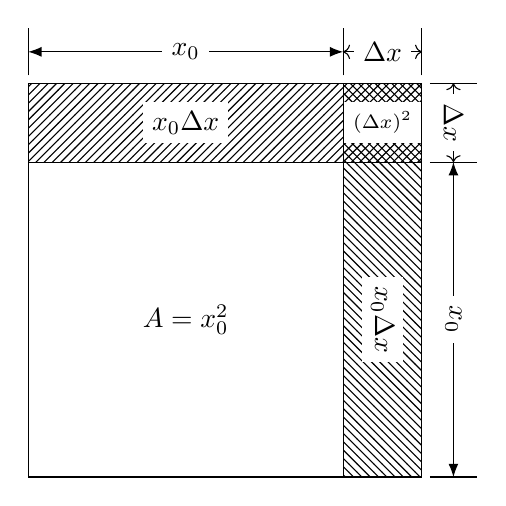
\begin{tikzpicture}
  \draw (0,0) rectangle (5, 5);
  \draw[pattern=north east lines] (0,4) rectangle (5, 5);
  \draw[pattern=north west lines] (4,0) rectangle (5, 5);

  \node at (2,2) {$A = x_0^2$};
  \node[fill=white] at (2,4.5) {$x_0 \Delta x$};
  \node[fill=white, rotate=-90] at (4.5,2) {$x_0 \Delta x$};
  \node[fill=white] at (4.5,4.5) {\scriptsize $(\Delta x)^2$};

  \draw (0, 5.1) -- (0, 5.7);
  \draw (4, 5.1) -- (4, 5.7);
  \draw (5, 5.1) -- (5, 5.7);
  \draw [Latex-Latex] (0, 5.4) -- (4,5.4);
  \node[fill=white] at (2,5.4) {$x_0$};
  \draw [<->] (4, 5.4) -- (5, 5.4);
  \node[fill=white] at (4.5,5.4) {$\Delta x$};

  \draw (5.1, 5) -- (5.7, 5);
  \draw (5.1, 4) -- (5.7, 4);
  \draw (5.1, 0) -- (5.7, 0);
  \draw [<->] (5.4, 5) -- (5.4, 4);
  \node[fill=white,rotate=-90] at (5.4,4.5) {$\Delta x$};
  \draw [Latex-Latex] (5.4, 4) -- (5.4, 0);
  \node[fill=white,rotate=-90] at (5.4,2) {$x_0$};
\end{tikzpicture}

    \caption{金属薄片面积受温度变化}
    \label{金属薄片面积受温度变化}
\end{figure}

\paragraph{}
$\Delta A$ 的第一部分 $2x_0\Delta x$ 是 $\Delta x$ 的线性函数,图中斜线的两个矩形面积之和;第二部分 $(\Delta x)^2$ 在图中带有交叉斜线的小正方形的面积。当 $\Delta x \to 0$ 时,第二部分 $(\Delta x)^2$ 比 $\Delta x$ 高阶无穷小,即 $(\Delta x)^2 = o(\Delta x)$。因此,如果边长改变的很微小,即 $|\Delta x|$ 很小时,面积的改变量 $\Delta A$ 可近似地用第一部分来代替。

\paragraph{}
\textbf{定义~~}设函数 $y = f(x)$ 在某区间内有定义,$x_0$ 及 $x_0 + \Delta x$ 在这区间内,如果增量

\begin{equation}
\Delta y = f(x_0 + \Delta x) - f(x_0)
\end{equation}

\paragraph{}
可表示为

\begin{equation}
\Delta y = A\Delta x + o(\Delta x),
\end{equation}

\paragraph{}
其中 $A$ 是不依赖于 $\Delta x$ 的常数,那么称函数 $y = f(x)$ 在点 $x_0$ 是\uwave{可微}的,而 $A\Delta x$ 叫做函数 $y = f(x)$ 在点 $x_0$ 相应于自变量增量 $\Delta x$ 的\uwave{微分},记作 $dy$,即

\begin{equation}
dy = A\Delta x.
\end{equation}

\paragraph{}
函数 $f(x)$ 在点 $x_0$ 可微的充分必要条件是函数 $f(x)$ 在点 $x_0$ 可导,且当 $f(x)$ 在点 $x_0$ 可微时,其微分一定是

\begin{equation}
dy = f'(x_0)\Delta x.
\end{equation}

\paragraph{}
当 $f'(x_0) \neq 0$ 时,有

\begin{equation}
\lim_{\Delta x \to 0} \frac{\Delta y}{dy} = \lim_{\Delta x \to 0} \frac{\Delta y}{f'(x_0) \Delta x} = \frac{1}{f'(x_0)}\lim_{\Delta x \to 0}\frac{\Delta y}{\Delta x} = 1.
\end{equation}

\paragraph{}
从而,当 $\Delta x \to 0$ 时,$\Delta y$ 与 $dy$ 是等价无穷小,这时有

\begin{equation}
\Delta y = dy + o(dy).
\end{equation}

即$dy$是$\Delta y$ 的\uwave{主部}。又由于$dy = f'(x_0) \Delta x$是$\Delta x$的线性函数,所以在$f'(x_0) \neq 0$的条件下,我们说$dy$是$\Delta y$的\uwave{线性主部}(当$\Delta x \to 0$)。

\paragraph{}
于是,在$f'(x_0) \neq 0$的条件下,以微分$dy = f'(x_0)\Delta x$近似代替增量$\Delta y = f(x_0+\Delta x) - f(x_0)$时,其误差为$o(dy)$。因此,在$|\Delta x|$很小时,有近似等式
\begin{equation}
  \Delta y \approx dy.
\end{equation}

\paragraph{}
函数$y=f(x)$在任意点$x$的微分,称为\uwave{函数的微分},记作$dy$或$df(x)$,即

\begin{equation}
  dy = f'(x)\Delta x.
\end{equation}

\paragraph{}
通常把自变量$x$的增量$\Delta x$称为\uwave{自变量的微分},记作$dx$,即$dx = \Delta x$。于是,函数$y=f(x)$的微分又可记作

\begin{equation}
  dy = f'(x)dx.
\end{equation}

从而有

\begin{equation}
  \frac{dy}{dx} = f'(x).
\end{equation}

\paragraph{}
也就是说,函数的微分$dy$与自变量的微分$dx$之商等于该函数的导数。因此,导数也叫做“\uwave{微商}”。

\subsection{微分的几何意义}
\paragraph{}
在直角坐标系中,函数$y = f(x)$的图形是一条曲线。对于某一固定的$x_0$值,曲线上有一个确定点$M(x_0,y_0)$,当自变量$x$有微小增量$\Delta x$时,就得到曲线上另一点$N(x_0 + \Delta x, y_0 + \Delta y)$。从图\figureref{differential_geometric_meaning}可知:

\begin{align*}
  MQ =&\; \Delta x, \\
  QN =&\; \Delta y.
\end{align*}

过点$M$作曲线的切线$MT$,它的倾角为$\alpha$,则
\begin{equation*}
  QP = MQ \bigcdot \tan{\alpha} = \Delta x \bigcdot f'(x_0),
\end{equation*}
即
\begin{equation*}
  dy = QP.
\end{equation*}

\begin{figure}[H]
  \centering
    % 微分的几何意义
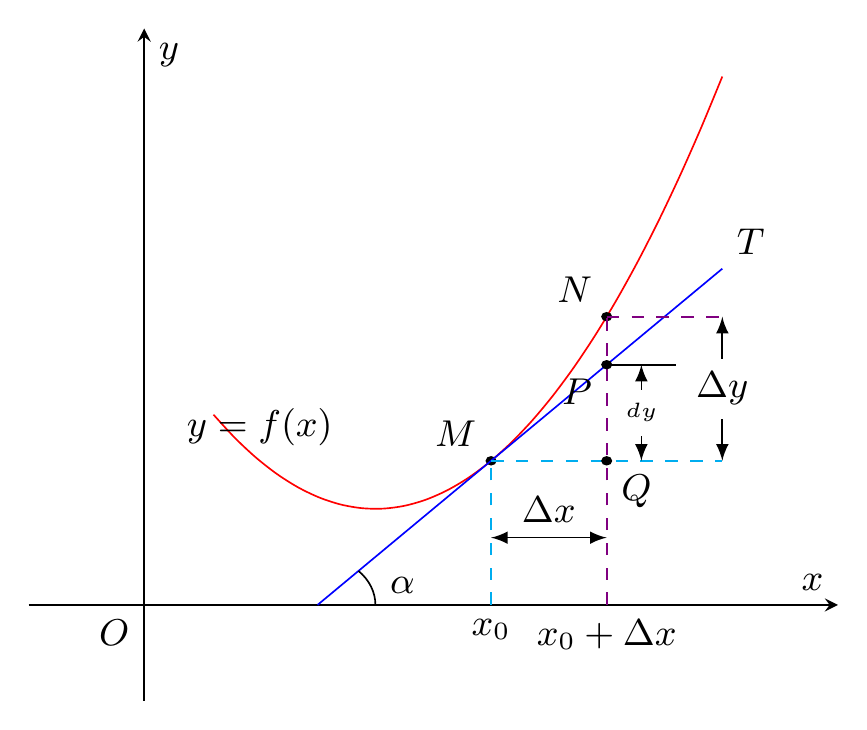
\begin{tikzpicture}[scale = 1.5]
  \begin{axis}[clip=false,xmin=-0.5, xmax=3,ymin=-0.5,ymax=3, grid=none,
    xtick=\empty, ytick=\empty, font=\small, axis lines=middle,
    smooth, xlabel={$x$}, ylabel={$y$}]

    % 曲线
    \addplot[draw=red,domain=0.3:2.5] {(x - 1)^2 + 0.5};
    \node [above] at (0.5,0.75) {$y = f(x)$};
    \draw[fill] (1.5,0.75) circle [radius=0.02];
    \draw[fill] (2,1.5) circle [radius=0.02];
    % 切线
    \addplot[draw=blue,domain=0.75:2.5] {x - 0.75};
    \node [above right] at (2.5,1.75) {$T$};

    % 辅助线和点
    \draw [dashed, draw=cyan] (1.5, 0) -- (1.5, 0.75);
    \draw [dashed, draw=cyan] (1.5, 0.75) -- (2.5, 0.75);
    \node [above left] at (1.5,0.75) {$M$};
    \node [below] at (1.5,0) {$x_0$};

    % \Delta x
    \draw [latex-latex] (1.5, 0.35) -- (2, 0.35);
    \node [above] at (1.75,0.35) {$\Delta x$};

    % \Delta y
    \draw [latex-latex] (2.5, 0.75) -- (2.5, 1.5);
    \node [fill=white] at (2.5,1.125) {$\Delta y$};

    % dy
    \draw (2, 1.25) -- (2.3, 1.25);
    \draw [latex-latex] (2.15, 0.75) -- (2.15, 1.25);
    \node [fill=white, font=\tiny] at (2.15,1) {$dy$};

    \draw [dashed, draw=violet] (2, 0) -- (2, 1.5);
    \draw [dashed, draw=violet] (2, 1.5) -- (2.5, 1.5);
    \node [above left] at (2,1.5) {$N$};
    \node [below] at (2,0) {$x_0 + \Delta x$};

    \draw[fill] (2,1.25) circle [radius=0.02];
    \node [below left] at (2,1.25) {$P$};

    \draw[fill] (2,0.75) circle [radius=0.02];
    \node [below right] at (2,0.75) {$Q$};

    % 倾角
    \draw (1,0) arc (0:45:0.25);
    \node [right] at (1,0.1) {$\alpha$};

    % 原点
    \node [below left] at (0,0) {$O$};
  \end{axis}
\end{tikzpicture}

    \caption{几何意义}
    \label{differential_geometric_meaning}
\end{figure}

\paragraph{}
由此可见,对于可微函数$y=f(x)$而言,当$\Delta y$是曲线$y=f(x)$上的点的纵坐标的增量时,$dy$就是曲线的切线上点的纵坐标的相应增量。

\paragraph{}
当$|\Delta x|$很小时,$|\Delta y - dy|$比$|\Delta x|$小得多。因此在点$M$的邻近,我们可以用切线段来近似代替曲线段。

\paragraph{}
在局部范围内用线性函数近似代替非线性函数,在几何上就是局部用切线段近似代替曲线段,这在数学上称为\textbf{非线性函数的局部线性化},这是微分学的基本思想方法之一。

\subsection{基本初等函数的微分公司与微分运算法则}
\paragraph{}
从函数的微分的表达式
\begin{equation}
  dy = f'(x)dx
\end{equation}
可以看出,要计算函数的微分,只要计算函数的导数,再乘以自变量的微分。因此可得如下的微分公司和微分运算法则。

\subsubsection{基本初等函数的微分公式}
\paragraph{}

\bgroup
\def\arraystretch{1.8}
\setlength\tabcolsep{1.8cm}
\begin{figure}[H]
\centering
  \begin{tabular}{c|c}
    \hline
    导数公式 & 微分公式 \\
    \hline
    $(x^\mu)' = \mu x^{\mu - 1}$ & $d(x^\mu) = \mu x^{\mu - 1}dx$ \\
    $(\sin{x})' = \cos{x}$ & $d(\sin{x}) = \cos{x}dx$ \\
    $(\cos{x})' = -\sin{x}$ & $d(\cos{x}) = -\sin{x}dx$ \\
    $(\tan{x})' = \sec^2{x}$ & $d(\tan{x}) = \sec^2{x}dx$ \\
    $(\cot{x})' = -\csc^2{x}$ & $d(\cot{x}) = -\csc^2{x}dx$ \\
    $(\sec{x})' = \sec{x}\tan{x}$ & $d(\sec{x}) = \sec{x}\tan{x}dx$ \\
    $(\csc{x})' = -\csc{x}\cot{x}$ & $d(\csc{x}) = -\csc{x}\cot{x}dx$ \\
    $(a^x)' = a^x\ln{a}$ & $d(a^x) = a^x\ln{a}dx$ \\
    $(e^x)' = e^x$ & $d(e^x) = e^xdx$ \\
    $(\log_a{x})' = \frac{1}{x\ln{a}}$ & $d(\log_a{x}) = \frac{1}{x\ln{a}}dx$ \\
    $(\ln{x})' = \frac{1}{x}$ & $d(\ln{x}) = \frac{1}{x}dx$ \\
    $(\arcsin{x})' = \frac{1}{\sqrt{1-x^2}}$ & $d(\arcsin{x}) = \frac{1}{\sqrt{1-x^2}}dx$ \\
    $(\arccos{x})' = -\frac{1}{\sqrt{1-x^2}}$ & $d(\arccos{x}) = -\frac{1}{\sqrt{1-x^2}}dx$ \\
    $(\arctan{x})' = \frac{1}{\sqrt{1+x^2}}$ & $d(\arctan{x}) = \frac{1}{\sqrt{1+x^2}}dx$ \\
    $(\arccot{x})' = -\frac{1}{\sqrt{1+x^2}}$ & $d(\arccot{x}) = -\frac{1}{\sqrt{1+x^2}}dx$ \\
    \hline
  \end{tabular}
\end{figure}
\egroup

\subsubsection{函数和、差、积、商的微分法则}
\paragraph{}
由函数和、差、积、商的求导法则,可推得相应的微分法则,表中$u = u(x), v = v(x)$都可导。

\bgroup
\def\arraystretch{2}
\setlength\tabcolsep{1.2cm}
\begin{figure}[H]
\centering
  \begin{tabular}{c|c}
    \hline
    函数和、差、积、商的求导法则 & 函数和、差、积、商的微分法则 \\
    \hline
    $(u \pm v)' = u' \pm v'$ & $d(u \pm v) = du \pm dv$ \\
    $(Cu)' = Cu'$ & $d(Cu) = Cdu$ \\
    $(uv)' = u'v + uv'$ & $d(uv) = vdu + udv$ \\
    $(\frac{u}{v})' = \frac{u'v - uv'}{v^2} \;(v \neq 0)$ & $d(\frac{u}{v}) = \frac{vdu - udv}{v^2} \;(v \neq 0)$ \\
    \hline
  \end{tabular}
\end{figure}
\egroup

\subsubsection{复合函数的微分法则}
\paragraph{}
设$y = f(u)$及$u = g(x)$都可导,则复合函数$y=f[g(x)]$的微分为
\begin{equation}
  dy = y'_x dx = f'(u)g'(x)dx.
\end{equation}
由于$g'(x)dx = du$,所以,复合函数$y = f[g(x)]$的微分公式也可以写成
\begin{equation}
  dy = f'(u)du \; \text{或} \; dy = y'_u du.
\end{equation}

\paragraph{}
由此可见,无论$u$是自变量还是中间变量,微分形式$dy = f'(u)du$保持不变,这一性质称为\textbf{微分形式不变性}。这性质表示,当变换自变量时,微分形式$dy = f'(u)du$并不改变。

\subsection{微分在近似计算中的应用}
\subsubsection{函数的近似计算}
\paragraph{}
在工程问题中,经常会遇到一些复杂的计算公式。如果直接用这些公式进行计算,那是很费力的。利用微分往往可以把一些复杂的计算公式用简单的近似公式来代替。
\paragraph{}
前面说过,如果$y = f(x)$在点$x_0$处的导数$f'(x_0) \neq 0$,且$|\Delta x|$很小时,我们有
\begin{equation}
  \label{函数的近似计算例子1}
  \Delta y \approx dy = f'(x_0)\Delta x.
\end{equation}
这个式子也可以写成
\begin{equation}
  \label{函数的近似计算例子2}
  \Delta y = f(x_0 + \Delta x) - f(x_0) \approx f'(x_0)\Delta x,
\end{equation}
或
\begin{equation}
  \label{函数的近似计算例子3}
  f(x_0 + \Delta x) \approx f(x_0) + f'(x_0)\Delta x.
\end{equation}
在\eqref{函数的近似计算例子3}式中令$x = x_0 + \Delta x$,即$\Delta x = x - x_0$,那么\eqref{函数的近似计算例子3}式可改写为
\begin{equation}
  \label{函数的近似计算例子4}
  f(x) \approx f(x_0) + f'(x_0)(x-x_0).
\end{equation}

\paragraph{}
如果$f(x_0)$与$f'(x_0)$都容易计算,那么可利用\eqref{函数的近似计算例子2}式来近似计算$\Delta y$,利用\eqref{函数的近似计算例子3}式来近似计算$f(x_0 + \Delta x)$,或利用\eqref{函数的近似计算例子4}式来近似计算$f(x)$。

\paragraph{}
这种近似计算的实质就是用$x$的线性函数$f(x_0) + f'(x_0)(x-x_0)$来近似表达函数$f(x)$。从导数的几何意义[图\figureref{differential_geometric_meaning}]可知道,这也就是用曲线$y=f(x)$在点$(x_0, f(x_0))$处的切线来近似代替该曲线(就切点邻近部分来说)。

\subsubsection{误差估计}
\paragraph{}
例如,计算圆钢的截面积$A$,可先用卡尺测量圆钢截面的直径$D$,然后根据公式$A = \frac{\pi}{4}D^2$算出$A$。

\paragraph{}
由于测量仪器的精度、测量的条件和测量的方法等各种因素的影响,测得的数据往往带有误差,而根据带有误差的数据计算,所得的结果也会有误差,我们把它叫做\uwave{间接测量误差}。

\paragraph{}
可以通过微分来估计间接测量误差。

\paragraph{}
如果某个量的精确值为$A$,它的近似值为$a$,那么$|A-a|$叫做$a$的\uwave{绝对误差}。而绝对误差与$|a|$的比值$\frac{|A-a|}{|a|}$叫做$a$的\uwave{相对误差}。

\paragraph{}
在实际工作中,某个量的精确值往往是无法知道的,于是绝对误差和相对误差也就无法求得。但是根据测量仪器的精度等因素,有时能够确定误差在某一个范围内。

\paragraph{}
如果某个量的精确值是$A$,测得它的近似值是$a$,又知道它的误差不超过$\delta_A$,即
\begin{equation}
  |A-a| \leq  \delta_A,
\end{equation}
那么$\delta_A$叫做测量$A$的\uwave{绝对误差限},而$\frac{\delta_A}{|a|}$叫做测量$A$的\uwave{相对误差限}。

\paragraph{}
一般的,根据直接测量的$x$值按公式$y=f(x)$计算$y$值时,如果已知测量$x$的绝对误差限是$\delta_x$,即
\begin{equation}
  |\Delta x| \leq \delta_x,
\end{equation}
那么,当$y' \neq 0$时,$y$的绝对误差
\begin{equation}
  |\Delta y| \approx |dy| = |y'| \bigcdot |\Delta x| \leq |y'| \bigcdot \delta_x,
\end{equation}
即$y$的绝对误差限约为
\begin{equation}
  \delta_y = |y'| \bigcdot \delta_x;
\end{equation}
$y$的相对误差限约为
\begin{equation}
  \frac{\delta_y}{|y|} = |\frac{y'}{y}| \bigcdot \delta_x.
\end{equation}

\paragraph{}
以后常把绝对误差限与相对误差限简称为\uwave{绝对误差}与\uwave{相对误差}。


  \newpage
  \part{微分中值定理与导数的应用}
  \section{微分中值定理}
    \paragraph{}
本章将应用导数来研究函数以及曲线的某些形态,并利用这些知识解决一些实际问题。为此,先介绍微分学的几个中值定理,它们是导数应用的理论基础。

\subsection{罗尔定理(Rolle's theorem)}
\paragraph{}
\textbf{费马引理\;}设函数$f(x)$在点$x_0$的某邻域$U(x_0)$内有定义,并且在$x_0$处可导,如果对任意的$x\in U(x_0)$,有
\begin{equation}
  f(x) \leq f(x_0) \;(\text{或} f(x) \geq f(x_0)),
\end{equation}
那么$f'(x_0) = 0$。

\begin{figure}[H]
  \centering
    \input{figure/Fermat‘s_theorem}
    \label{Fermat‘s_theorem}
    \caption{费马引理}
\end{figure}

\paragraph{}
通常称导数等于零的点为函数的\uwave{驻点}(或\uwave{稳定点},\uwave{临界点})。

\paragraph{}
\textbf{罗尔定理\;}如果函数$f(x)$满足
\begin{enumerate}
  \item 在闭区间$[a,b]$上连续;
  \item 在开区间$(a,b)$内可导;
  \item 在区间端点处的函数值相等,即$f(a)=f(b)$,
\end{enumerate}
那么在$(a,b)$内至少有一点$\xi(a < \xi < b)$,使得$f'(\xi) = 0$。

\subsection{拉格朗日中值定理(Lagrange's mean value theorem)}
\subsubsection{定理}
\paragraph{}
罗尔定理中$f(a)=f(b)$这个条件是相当特殊的,它使罗尔定理的应用受到限制。如果把该条件取消,但仍保留其余两个条件,并相应的改变结论,那么得到微分学中十分重要的拉格朗日中值定理。

\paragraph{}
\textbf{拉格朗日中值定理\;}如果函数$f(x)$满足
\begin{enumerate}
  \item 在闭区间$[a,b]$上连续;
  \item 在开区间$(a,b)$内可导,
\end{enumerate}
那么在$(a,b)$内至少有一点$\xi(a < \xi < b)$,使等式
\begin{equation}
  f(b) - f(a) = f'(\xi)(b-a)
\end{equation}
成立。

\begin{figure}[H]
  \centering
    \input{figure/Lagrange‘s_mean_value_theorem}
    \caption{拉格朗日中值定理}
    \label{Lagrange‘s mean value theorem}
\end{figure}

\paragraph{}
从图\figureref{Lagrange‘s mean value theorem}中看出,在罗尔定理中,由于$f(a)=f(b)$,弦$AB$是平行于$x$轴的,因此点$C$处的切线实际上也平行于弦$AB$。由此可见,罗尔定理是拉格朗日中值定理的特殊情形。

\subsubsection{证明}
\paragraph{}
\textbf{证明前的准备\;}使用罗尔定理来证明拉格朗日中值定理。

\paragraph{}
在拉格朗日中值定理中,函数$f(x)$不一定具备$f(a)=f(b)$这个条件,为此我们设想构造一个与$f(x)$有密切联系的函数$\varphi(x)$(称为\uwave{辅助函数}),使$\varphi(x)$满足条件$\varphi(a) = \varphi(b)$。然后应用罗尔定理。

\paragraph{}
从图\figureref{Lagrange‘s mean value theorem}中看到,有向线段$NM$的值是与$x$有关联的函数,把它表示为$\varphi(x)$,它与$f(x)$有密切的联系,且当$x=a$及$x=b$时,点$M$与点$N$重合,即有$\varphi(a)=\varphi(b)=0$。为求得函数$\varphi(x)$的表达式,设直线$AB$的方程为$y=L(x)$,则

\begin{equation*}
  L(x) = f(a) + \frac{f(b) - f(a)}{b - a}(x-a)
\end{equation*}

由于点$M$、$N$的纵坐标依次为$f(x)$及$L(x)$,故表示有向线段$NM$的值的函数

\begin{equation*}
  \varphi(x) = f(x) - L(x) = f(x) - f(a) - \frac{f(b) - f(a)}{b - a}(x - a).
\end{equation*}

\paragraph{}
\textbf{定理的证明\;}引进辅助函数

\begin{equation}
  \varphi(x) = f(x) - f(a) - \frac{f(b) - f(a)}{b - a}(x - a).
\end{equation}

容易验证函数$\varphi(x)$适合罗尔定理的条件:$\varphi(a) = \varphi(b) = 0$;$\varphi(x)$在闭区间$[a,b]$上连续,在开区间$(a,b)$内可导,且

\begin{equation}
  \varphi'(x) = f'(x) - \frac{f(b) - f(a)}{b - a}.
\end{equation}

根据罗尔定理,可知在$(a,b)$内至少有一点$\xi$,使$\varphi'(\xi) = 0$,即

\begin{equation}
  f'(\xi) - \frac{f(b) - f(a)}{b - a} = 0.
\end{equation}

由此得
\begin{equation}
  \frac{f(b) - f(a)}{b - a} = f'(\xi).
\end{equation}

即

\begin{equation}
  \label{拉格朗日中值公式}
  f(b) - f(a) = f'(\xi)(b - a).
\end{equation}

定理证毕。

\paragraph{}
公式\eqref{拉格朗日中值公式}对于$b<a$也成立,该式叫做\uwave{拉格朗日中值公式}

\subsubsection{推论}
\paragraph{}
拉格朗日中值定理在微分学中占有重要地位,有时也称该定理为\uwave{微分中值定理}。以及推导出一个重要推论,对后面积分学很有帮助。

\paragraph{}
如果函数$f(x)$在某一区间上是一个常数,那么$f(x)$在该区间上的导数恒为$0$。它的逆命题也成立:

\paragraph{}
\textbf{推论\;}如果函数$f(x)$在区间$I$上的导数恒为$0$,那么$f(x)$在区间$I$上是一个常数。

\subsection{柯西中值定理(Cauchy's mean value theorem)}
\paragraph{}
\begin{figure}[H]
  \centering
    \input{figure/Cauchy‘s_mean_value_theorem}
    \caption{柯西中值定理}
    \label{Cauchy‘s mean value theorem}
\end{figure}

\paragraph{}
设$AB$由参数方程
\begin{equation}
  \left\{
    \begin{array}{l}
      X = F(x), \\
      Y = f(x)
    \end{array}
    \;(a \leq x \leq b)
  \right.
\end{equation}
表示(图\figureref{Cauchy‘s mean value theorem}),其中$x$为参数,那么曲线上点$(X,Y)$处的切线的斜率为
\begin{equation}
  \frac{dY}{dX}=\frac{f'(x)}{F'(x)}
\end{equation}
弦$AB$的斜率为
\begin{equation}
  \frac{f(b)-f(a)}{F(b)-F(a)}
\end{equation}
假定点$C$对应于参数$x=\xi$,那么曲线上点$C$处的切线平行于弦$AB$,可表示为
\begin{equation}
  \frac{f(b)-f(a)}{F(b)-F(a)} = \frac{f'(x)}{F'(x)}
\end{equation}
因此

\paragraph{}
\textbf{柯西中值定理\;}如果函数$f(x)$及$F(x)$满足
\begin{enumerate}
  \item 在闭区间$[a,b]$上连续;
  \item 在开区间$(a,b)$内可导;
  \item 对任一$x \in (a,b), F'(x) \neq 0$,
\end{enumerate}
那么在$(a,b)$内至少有一点$\xi$,使等式
\begin{equation}
  \frac{f(b)-f(a)}{F(b)-F(a)} = \frac{f'(\xi)}{F'(\xi)}
\end{equation}
成立。

  \section{洛必达法则(L'Hôpital's rule)}
    \subsection{洛必达法则}
\paragraph{}
如果当$x \to a$(或$x\to \infty$)时,两个函数$f(x)$与$F(x)$都趋于$0$或$\infty$,那么极限$\displaystyle \lim_{\substack{x \to a \\ (x \to \infty)}} \frac{f(x)}{F(x)}$可能存在、也可能不存在。通常把这种极限叫做\uwave{未定式},并分别简记为$\frac{0}{0}$或$\frac{\infty}{\infty}$。

\paragraph{}
对于这类极限,即使它存在也不能用“商的极限等于极限的商”这一法则。下面根据柯西中值定理推出这类极限的一种简便且重要的方法。

\subsubsection{定理1}
\paragraph{}
\textbf{定理1\;}$x \to a$时的未定式$\frac{0}{0}$的情形,设:
\begin{enumerate}
  \item 当$x \to a$时,函数$f(x)$及$F(x)$都趋于零;
  \item 在点$a$的某去心邻域内,$f'(x)$及$F'(x)$都存在且$F'(x) \neq 0$;
  \item $\displaystyle \lim_{x \to a}\frac{f'(x)}{F'(x)}$存在(或为$\infty$),
\end{enumerate}
那么
\begin{equation}
  \lim_{x \to a}\frac{f(x)}{F(x)} = \lim_{x \to a} \frac{f'(x)}{F'(x)}.
\end{equation}

\paragraph{}
这种在一定条件下通过分子分母分别求导再求极限来确定未定式的值的方法称为\uwave{洛必达法则}。

\paragraph{}
\textbf{证\;}因为求$\frac{f(x)}{F(x)}$当$x\to a$时的极限与$f(a)$及$F(a)$无关,所以可以假定$f(a) = F(a) = 0$,于是由条件$1$、$2$知道,$f(x)$及$F(x)$在点$a$的某一邻域内是连续的。设$x$是这邻域内的一点,那么在以$x$及$a$为端点的区间上,柯西中值定理的条件均满足,因此有

\begin{equation}
  \frac{f(x)}{F(x)} = \frac{f(x) - f(a)}{F(x) - F(a)} = \frac{f'(\xi)}{F'(\xi)} \; \text{($\xi$在$x$与$a$之间)}.
\end{equation}
令$x \to a$,并对上式两端求极限,注意到$x\to a$时$\xi \to a$,再根据条件$3$便得到证明的结论。

\subsubsection{定理2}
\paragraph{}
\textbf{定理2\;}$x \to \infty$时的未定式$\frac{\infty}{\infty}$的情形,设:
\begin{enumerate}
  \item 当$x \to \infty$时,函数$f(x)$及$F(x)$都趋于零;
  \item 当$|x|>N$时$f'(x)$与$F'(x)$都存在,且$F'(x) \neq 0$;
  \item $\displaystyle \lim_{x \to \infty}\frac{f'(x)}{F'(x)}$存在(或为$\infty$),
\end{enumerate}
那么
\begin{equation}
  \lim_{x\to \infty}\frac{f(x)}{F(x)} = \lim_{x\to \infty}\frac{f'(x)}{F'(x)}.
\end{equation}

  \section{泰勒公式(Taylor's theorem)}
    \input{3_Taylor‘s_theorem}
  \section{函数的单调性与曲线的凹凸性}
    \subsection{函数单调性的判定法}
\paragraph{}
如果函数$y=f(x)$在$[a,b]$上单调增加(单调减少),那么它的图形是一条沿$x$轴正向上升(下降)的曲线。

\begin{figure}[H]
\centering
  %------- 第1行 -------
  \begin{subfigure}[t]{0.48\linewidth}
    \centering
      % 单调增加
\begin{tikzpicture}[scale=0.8]
  \begin{axis}[clip=false,xmin=0, xmax=6,ymin=0,ymax=4, grid=none,
    xtick=\empty, ytick=\empty, axis lines=middle,
    smooth, xlabel={$x$}, ylabel={$y$}]

    % 曲线
    \addplot[draw=red,domain=1.5:4.5] {(x - 1)^5 / (4 * x^3) + 1.5};

    % 端点辅助线
    \draw [dashed] (1.5,0) -- (1.5,1.5);
    \draw [dashed] (4.5,0) -- (4.5,2.94);

    % 端点标记
    \node [left] at (1.5,1.5) {$A$};
    \node [below] at (1.5,0) {$a$};
    \node [right] at (4.5,2.94) {$B$};
    \node [below] at (4.5,0) {$b$};

    % y = f(x)
    \node [left] at (4,2.44) {$y=f(x)$};

    % 切线, dx/dy = 0.444~
    \draw [fill] (3,1.79) circle [radius=0.03];
    \draw (1.3, 1.03) -- (3, 1.79) -- (4.7, 2.54);

    % 原点
    \node [below left] at (0,0) {$O$};
  \end{axis}
\end{tikzpicture}

    \subcaption{单调增加}
  \end{subfigure}
  \begin{subfigure}[t]{0.48\linewidth}
    \centering
      % 单调增加
\begin{tikzpicture}[scale=0.8]
  \begin{axis}[clip=false,xmin=0, xmax=6,ymin=0,ymax=4, grid=none,
    xtick=\empty, ytick=\empty, axis lines=middle,
    smooth, xlabel={$x$}, ylabel={$y$}]

    % 曲线
    \addplot[draw=red,domain=1.5:4.5] {(-x+1)^5 / (4*x^3) + 2.5};

    % 端点辅助线
    \draw [dashed] (1.5,0) -- (1.5,2.5);
    \draw [dashed] (4.5,0) -- (4.5,1.06);

    % 端点标记
    \node [left] at (1.5,2.5) {$A$};
    \node [below] at (1.5,0) {$a$};
    \node [right] at (4.5,1.06) {$B$};
    \node [below] at (4.5,0) {$b$};

    % y = f(x)
    \node [left] at (4,1.55) {$y=f(x)$};

    % 切线, dx/dy = -0.444~
    \draw [fill] (3,2.2) circle [radius=0.03];
    \draw (1.3,2.94) -- (3,2.2) -- (4.7,1.45);

    % 原点
    \node [below left] at (0,0) {$O$};
  \end{axis}
\end{tikzpicture}

    \subcaption{单调减少}
  \end{subfigure}
  \caption{函数单调性}
  \label{函数单调性}
\end{figure}

\paragraph{}
由拉格朗日中值定理和定义可证明:

\paragraph{}
\textbf{定理1\;}设函数$y=f(x)$在$[a,b]$上连续,在$(a,b)$内可导:
\begin{enumerate}
  \item 如果在$(a,b)$内$f'(x) > 0$,那么函数$y=f(x)$在$[a,b]$上单调增加;
  \item 如果在$(a,b)$内$f'(x) < 0$,那么函数$y=f(x)$在$[a,b]$上单调减少;
\end{enumerate}

\subsection{曲线的凹凸性与拐点}
\subsubsection{凹凸性}
\paragraph{}
\textbf{定义\;}设$f(x)$在区间$I$上连续,如果对$I$上任意两点$x_1,x_2$恒有
\begin{equation}
  f(\frac{x_1+x_2}{2}) < \frac{f(x_1) + f(x_2)}{2},
\end{equation}
那么称$f(x)$在$I$上的图形是\uwave{(向上)凹的(或凹弧)};如果恒有
\begin{equation}
  f(\frac{x_1+x_2}{2}) > \frac{f(x_1)+f(x_2)}{2},
\end{equation}
那么称$f(x)$在$I$上的图形是\uwave{(向上)凸的(或凸弧)}。

\paragraph{}

\begin{figure}[H]
\centering
  %------- 第1行 -------
  \begin{subfigure}[t]{0.48\linewidth}
    \centering
      % 函数凹弧
\begin{tikzpicture}[scale=0.8]
  \begin{axis}[clip=false,xmin=0, xmax=6,ymin=0,ymax=6, grid=none,
    xtick=\empty, ytick=\empty, axis lines=middle,
    smooth, xlabel={$x$}, ylabel={$y$}]

    % 曲线
    \addplot[draw=red,domain=1.3:4.7] {(x-3)^2/x + 2};
    % f'(x) = (2*(x-3)*x - (x-3)^2)) / x^2

    % 端点辅助线
    \draw [dashed] (1.8,0) -- (1.8,2.8);
    \draw [dashed] (4.2,0) -- (4.2,2.34);

    % 曲线端点的标记
    \node [below] at (1.8,0) {$x_1$};
    \node [below left] at (1.8,2.8) {$f(x_1)$};
    \node [below] at (4.2,0) {$x_2$};
    \node [below right] at (4.2,2.34) {$f(x_2)$};
    \node [below] at (3,0) {$\frac{x_1+x_2}{2}$};

    % 割线:y - 2.8 = -0.19 * (x - 1.8)
    \draw [fill] (3,2.57) circle [radius=0.03];
    \draw (1.8,2.8) -- (4.2,2.34);
    % 割线标记
    \node [above] at (3,2.7) {$\frac{f(x_1)+f(x_2)}{2}$};
    \draw [dashed] (3,2.57) -- (3,0);

    % 曲线上的 x=3,中点
    \node [fill=white,below, inner sep=1.5] at (3,1.8) {$f(\frac{x_1+x_2}{2})$};
    \draw [fill] (3,2) circle [radius=0.03];

    % 原点
    \node [below left] at (0,0) {$O$};
  \end{axis}
\end{tikzpicture}

    \subcaption{凹弧}
  \end{subfigure}
  \begin{subfigure}[t]{0.48\linewidth}
    \centering
      % 函数凹弧一阶、二阶导函数
\begin{tikzpicture}[scale=0.8]
  \begin{axis}[clip=false,xmin=0, xmax=6,ymin=-5,ymax=10, grid=none,
    xtick=\empty, ytick=\empty, axis lines=middle,
    smooth, xlabel={$x$}, ylabel={$y$}]

    % 一阶导函数
    \addplot[draw=red,domain=1.3:4.7] {1 - 9 * x^(-2)};
    % 二阶导函数
    \addplot[draw=blue,domain=1.3:4.7] {18 * x^(-3)};

    \node [left] at (1.5,-3) {$f'(x)$};
    \node [left] at (1.5,5.33) {$f''(x)$};

    % 原点
    \node [below left] at (0,0) {$O$};
  \end{axis}
\end{tikzpicture}

    \subcaption{一阶和二阶导函数}
  \end{subfigure}
  %------- 第2行 -------
  \begin{subfigure}[t]{0.48\linewidth}
    \centering
      % 函数凸弧弧
\begin{tikzpicture}[scale=0.8]
  \begin{axis}[clip=false,xmin=0, xmax=6,ymin=0,ymax=6, grid=none,
    xtick=\empty, ytick=\empty, axis lines=middle,
    smooth, xlabel={$x$}, ylabel={$y$}]

    % 曲线
    \addplot[draw=red,domain=1.3:4.7] {-(x-3)^2/x + 3.5};
    % f'(x) = -(2*(x-3)*x - (x-3)^2)) / x^2

    % 端点辅助线
    \draw [dashed] (1.8,0) -- (1.8,2.7);
    \draw [dashed] (4.2,0) -- (4.2,3.16);

    % 曲线端点的标记
    \node [below] at (1.8,0) {$x_1$};
    \node [above left] at (1.8,2.7) {$f(x_1)$};
    \node [below] at (4.2,0) {$x_2$};
    \node [above right] at (4.2,3.16) {$f(x_2)$};
    \node [below] at (3,0) {$\frac{x_1+x_2}{2}$};

    % 割线:y - 2.7 = 0.19 * (x - 1.8)
    \draw [fill] (3,2.93) circle [radius=0.03];
    \draw (1.8,2.7) -- (4.2,3.16);

    % 曲线上的 x=3,中点
    \node [above] at (3,3.6) {$f(\frac{x_1+x_2}{2})$};
    \draw [fill] (3,3.5) circle [radius=0.03];

    % 割线标记
    \node [fill=white,below,inner sep=1.5] at (3,2.7) {$\frac{f(x_1)+f(x_2)}{2}$};
    \draw [dashed] (3,3.5) -- (3,0);

    % 原点
    \node [below left] at (0,0) {$O$};
  \end{axis}
\end{tikzpicture}

    \subcaption{凸弧}
  \end{subfigure}
  \begin{subfigure}[t]{0.48\linewidth}
    \centering
      % 函数凸弧一阶、二阶导函数
\begin{tikzpicture}[scale=0.8]
  \begin{axis}[clip=false,xmin=0, xmax=6,ymin=-9,ymax=6, grid=none,
    xtick=\empty, ytick=\empty, axis lines=middle,
    smooth, xlabel={$x$}, ylabel={$y$}]

    % 一阶导函数
    \addplot[draw=red,domain=1.3:4.7] {-1 + 9 * x^(-2)};
    % 二阶导函数
    \addplot[draw=blue,domain=1.3:4.7] {-18 * x^(-3)};

    \node [left] at (1.5,3) {$f'(x)$};
    \node [left] at (1.5,-5.33) {$f''(x)$};

    % 原点
    \node [below left] at (0,0) {$O$};
  \end{axis}
\end{tikzpicture}

    \subcaption{一阶和二阶导函数}
  \end{subfigure}
  \caption{函数凹凸性}
  \label{函数凹凸性}
\end{figure}

\paragraph{}
由拉格朗日中值定理和定义可证明:

\paragraph{}
\textbf{定理2\;}设$f(x)$在$[a,b]$上连续,在$(a,b)$内具有一阶和二阶导数,那么
\begin{enumerate}
  \item 若在$(a,b)$内$f''(x) > 0$,则$f(x)$在$[a,b]$上的图形是凹的;
  \item 若在$(a,b)$内$f''(x) < 0$,则$f(x)$在$[a,b]$上的图形是凸的。
\end{enumerate}

\subsubsection{拐点}
\paragraph{}
设$y=f(x)$在区间$I$上连续,$x_0$是$I$的内点。如果曲线$y=f(x)$在经过点$(x_0,f(x_0))$时,曲线的凹凸性改变了,那么就称点$(x_0,f(x_0))$为这曲线的\uwave{拐点}。

\paragraph{}
由$f''(x)$的符号可以判定曲线的凹凸性,因此,如果$f''(x)$在$x_0$的左右两侧邻近异号,那么点$(x_0,f(x_0))$就是曲线的一个拐点。

\paragraph{}
除此之外,$f(x)$的二阶导数不存在的点,也有可能是$f''(x)$的符号发生变化的分界点。因此,找拐点的步骤:
\begin{enumerate}
  \item 求$f''(x)$;
  \item 令$f''(x)=0$,解出这方程在区间$I$内的实根,并求出在区间$I$内$f''(x)$不存在的点;
  \item 对于$2$中求出的每一个实根或二阶导数不存在的点$x_0$,检查$f''(x)$在$x_0$左、右两侧邻近的符号,当两侧的符号相反时,点$(x_0,f(x_0))$是拐点,当两侧的符号相同时,点$(x_0,f(x_0))$不是拐点。
\end{enumerate}

  \section{函数的极值与最大值最小值}
    \subsection{函数的极值及其求法}
\subsubsection{定义}
\paragraph{}
\textbf{定义\;}设函数$f(x)$在点$x_0$的某邻域$U(x_0)$内有定义,如果对于去心邻域$\mathring{U}(x_0)$内的任一$x$,有
\begin{equation}
  f(x) < f(x_0) \;\; \text{(或$f(x) > f(x_0)$)},
\end{equation}
那么就称$f(x_0)$是函数$f(x)$的一个\uwave{极大值}(或\uwave{极小值})。

\paragraph{}
函数的极大值与极小值统称为函数的\uwave{极值},使函数取得极值的点称为\uwave{极值点}。极值的概念是局部性的。

\subsubsection{定理}
\paragraph{}
\textbf{定理1(必要条件)\;}设函数$f(x)$在$x_0$处可导,且在$x_0$处取得极值,那么$f'(x_0)=0$。

\paragraph{}
反过来确不一定,比如:$f(x)=x^3$的导数$f'(x)=3x^2, f'(0) = 0$。

\paragraph{}
\textbf{定理2(第一充分条件)\;}设函数$f(x)$在$x_0$处连续,且在$x_0$的某去心邻域$\mathring{U}(x_0,\delta)$内可导。
\begin{enumerate}
  \item 若$x\in (x_0 - \delta, x_0)$时,$f'(x) > 0$,而$x \in (x_0,x_0+\delta)$时,$f'(x) < 0$,则$f(x)$在$x_0$处取得极大值;
  \item 若$x\in(x_0-\delta,x_0)$时,$f'(x)<0$,而$x\in(x_0,x_0+\delta)$时,$f'(x)>0$,则$f(x)$在$x_0$处取得极小值;
  \item 若$x\in\mathring{U}(x_0,\delta)$时,$f'(x)$的符号保持不变,则$f(x)$在$x_0$处没有极值。
\end{enumerate}

\paragraph{}
\textbf{定理3(第二充分条件)\;}设函数$f(x)$在$x_0$处具有二阶导数且$f'(x_0)=0, f''(x_0) \neq 0$,那么
\begin{enumerate}
  \item 当$f''(x_0)<0$时,函数$f(x)$在$x_0$处取得极大值;
  \item 当$f''(x_0)>0$时,函数$f(x)$在$x_0$处取得极小值。
\end{enumerate}

\subsection{最大值最小值问题}
\paragraph{}
在工农业生产、工程技术及科学实验中,常常会遇到这样一类问题:在一定条件下,怎样使“产品最多”、“用料最省”、“成本最低”、“效率最高”等问题,这类问题在数学上有时可归纳为求某一函数(通常称为\uwave{目标函数})的最大值或最小值。

\paragraph{}
最大值和最小值的方法:
\begin{enumerate}
  \item 求出$f(x)$在$(a,b)$内的驻点$x_1,x_2, \cdots, x_m$及不可导点$x'_1,x'_2,\cdots,x'_n$;
  \item 计算$f(x_i)(i=1,2,\cdots,m), \; f(x'_j)(j=1,2,\cdots,n)$及$f(a),f(b)$;
  \item 比较$2$中诸值的大小,其中最大的便是$f(x)$在$[a,b]$上的最大值,最小的便是$f(x)$在$[a,b]$上的最小值。
\end{enumerate}

\paragraph{}
应用例子:
\begin{enumerate}
  \item 折射定律
  \item 经济学的边际成本、边际收入和边际利润
\end{enumerate}

  \section{函数图形的描绘}
    \subsection{函数图形的描绘}
\paragraph{}
借助于一阶导数的符号,可以确定函数图形在哪个区间上上升,哪个区间上下降,在什么地方有极值点。
\paragraph{}
借助于二阶导数的符号,可以确定函数图形在哪个区间上为凹,在哪个区间上为凸,在什么地方有拐点。知道函数图形的升降、凹凸以及极值点和拐点后,也就可以掌握函数的性态。

\paragraph{}
\begin{enumerate}
  \item 确定定义域,及函数具有的特性(奇偶性、周期性等),并求出一阶导数$f'(x)$和二阶导数$f''(x)$;
  \item 求出一阶导数和二阶导数在定义域的全部零点,并求出函数$f(x)$的间断点及$f'(x)$和$f''(x)$不存在的点,划分函数的定义域;
  \item 确定这些部分区间内$f'(x)$和$f''(x)$的符号,并由此确定函数图形的升降和凹凸,极值点和拐点;
  \item 算出$f'(x)$和$f''(x)$的零点以及不存在的点所对应的函数值,定出图形上相应的点;为了把图形描绘得准确些,有时还需要补充一些点;然后结合第$3$、$4$步中得到的结果,联结这些点画出函数$y=f(x)$的图形。
\end{enumerate}

\subsection{例子}
\paragraph{}
\textbf{例子1\;}画出函数$y=x^3-x^2-x+1$的图形

\paragraph{}
\textbf{解}

\bgroup
\def\arraystretch{1.5}
\setlength\tabcolsep{0.3cm}
\begin{figure}[H]
\centering
  \begin{tabular}{c|c|c|c|c|c|c|c}
    \hline
    $x$ & $(-\infty,-\frac{1}{3})$ & $-\frac{1}{3}$ & $(-\frac{1}{3},\frac{1}{3})$ & $\frac{1}{3}$
    & $(\frac{1}{3},1)$ & $1$ & $(1,+\infty)$ \\
    \hline
    $f'(x)$ & $+$ & $0$ & $-$ & $-$ & $-$ & $0$ &$+$ \\
    \hline
    $f''(x)$ & $-$ & $-$ & $-$ & $0$ & $+$ & $+$ & $+$ \\
    \hline
    $y=f(x)\text{的图形}$ &
    {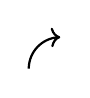
\begin{tikzpicture}[scale=0.4,thick]
      \draw [->,domain=180:90] plot ({cos(\x)}, {sin(\x)});
    \end{tikzpicture}} & 极大 &
    {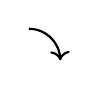
\begin{tikzpicture}[scale=0.4,thick]
      \draw [->,domain=90:0] plot ({cos(\x)}, {sin(\x)});
    \end{tikzpicture}} & 拐点 &
    {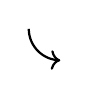
\begin{tikzpicture}[scale=0.4,thick]
      \draw [->,domain=180:270] plot ({cos(\x)}, {sin(\x)});
    \end{tikzpicture}} & 极小 &
    {
\begin{tikzpicture}[scale=0.4,thick]
      \draw [->,domain=-90:0] plot ({cos(\x)}, {sin(\x)});
    \end{tikzpicture}} \\
    \hline
  \end{tabular}
\end{figure}
\egroup

  \section{曲率}
    \subsection{弧微分}
\paragraph{}
设函数$f(x)$在区间$(a,b)$内具有连续导数。在曲线$y=f(x)$上取固定点$M_0(x_0,y_0)$作为度量弧长的基点,并规定依$x$增大的方向作为曲线的正向。对曲线上任一点$M(x,y)$,规定有向弧段$\overarc{M_0M}$的值$s$(简称为弧$s$);$s$的绝对值等于这弧段的长度,当有向弧段$\overarc{M_0M}$的方向与曲线的正向一致时$s>0$,相反时$s<0$。显然,弧$s$与$x$存在函数关系:$s=s(x)$,而且$s(x)$是$x$的单调增加函数。下面求$s(x)$的导数及微分。

\paragraph{}

\begin{figure}[H]
\centering
  % 弧微分
\begin{tikzpicture}[scale=0.8]
  \begin{axis}[clip=false,xmin=0, xmax=8,ymin=0,ymax=8, grid=none,
    xtick=\empty, ytick=\empty, axis lines=middle,
    smooth, xlabel={$x$}, ylabel={$y$}]

    % 曲线
    \addplot[draw=red,domain=1:7] {(x-3)^2/4 + 2};

    % 辅助线
    \draw [dashed] (2,0) -- (2,2.25);
    \draw [dashed] (5,0) -- (5,3);
    \draw [dashed] (6,0) -- (6,4.25);
    \draw [dashed] (5,3) -- (6,3);

    % 标记
    \node [below] at (2,0) {$x_0$};
    \node [above] at (2,2.25) {$M_0$};
    \node [below] at (5,0) {$x$};
    \node [above left] at (5,3) {$M$};
    \node [below] at (6,0) {$x+\Delta x$};
    \node [above left] at (6,4.25) {$M'$};

    \node [below] at (5.5,3) {$\Delta x$};
    \node [right] at (6,3.63) {$\Delta y$};

    % 原点
    \node [below left] at (0,0) {$O$};
  \end{axis}
\end{tikzpicture}

  \caption{弧微分}
  \label{弧微分}
\end{figure}

\paragraph{}
\textbf{推导\;}设$x, x+\Delta x$为$(a,b)$内两个邻近的点,它们在曲线$y=f(x)$上的对应点为$M, M'$(图\figureref{弧微分}),并设对应于$x$的增量$\Delta x$,弧$s$的增量为$\Delta s$,那么

\begin{equation}
  \Delta s = \overarc{M_0M'} - \overarc{M_0M} = \overarc{MM'}.
\end{equation}

于是
\begin{align}
\begin{split}
  \big(\frac{\Delta s}{\Delta x}\big)^2 = \big(\frac{\overarc{MM'}}{\Delta x}\big)^2 =&\; \big(\frac{\overarc{MM'}}{|MM'|}\big)^2 \bigcdot \frac{|MM'|^2}{(\Delta x)^2} \\
  =&\; \big(\frac{\overarc{MM'}}{|MM'|}\big)^2 \bigcdot \frac{(\Delta x)^2+(\Delta y)^2}{(\Delta x)^2} \\
  =&\; \big(\frac{\overarc{MM'}}{|MM'|}\big)^2\big[1+\big(\frac{\Delta y}{\Delta x}\big)^2\big],
\end{split}
\end{align}
得
\begin{equation}
  \frac{\Delta s}{\Delta x} = \pm \sqrt{\rule{0pt}{5ex} \big(\frac{\overarc{MM'}}{|MM'|}\big)^2\big[1+\big(\frac{\Delta y}{\Delta x}\big)^2\big]}.
\end{equation}
令$\Delta x \to 0$取极限,由于$\Delta x \to 0$时,$M' \to M$,这时弧的长度与弦的长度之比的极限等于$1$,即

\begin{equation}
  \lim_{M'\to M}\frac{\overarc{MM'}}{|MM'|}=1,
\end{equation}
又
\begin{equation}
  \lim_{\Delta x \to 0} \frac{\Delta y}{\Delta x} = y',
\end{equation}
因此得
\begin{equation}
  \frac{ds}{dx} = \pm \sqrt{1+y'^2}.
\end{equation}
由于$s=s(x)$是单调增加函数,从而根号前应取正号,于是有
\begin{equation}
  \label{弧微分公式}
  ds=\sqrt{1+y'^2}dx.
\end{equation}
这就是\uwave{弧微分公式}。

\subsection{曲率及其计算公式}
\paragraph{}
研究曲线的弯曲程度。曲线弧的弯曲程度与\uwave{切线转过的角度{$\varphi$}}和\uwave{弧段的长度}有关。

\begin{figure}[H]
\centering
  %------- 第1行 -------
  \begin{subfigure}[t]{0.45\linewidth}
    \centering
      % 曲率,例子 1
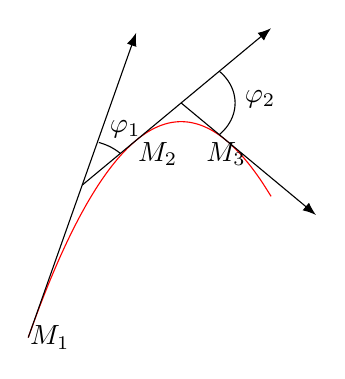
\begin{tikzpicture}[scale=1]
  \begin{axis}[clip=false,xmin=0, xmax=6,ymin=0,ymax=6, grid=none,
    xtick=\empty, ytick=\empty, axis lines=none, smooth]

    % 曲线
    \addplot[draw=red,domain=1.3:4] {-(x - 3)^2 + 4.5};

    % 导数
    % y' = -2*(x-3)

    % 切线1:y = 3.4 * x - 2.81
    \draw [-Latex] (1.3,1.61) -- (2.5,5.69);
    % 切线2:y = x + 1.75
    \draw [-Latex] (1.9,3.65) -- (2.5,4.25) -- (4,5.75);
    % 切线3:y = -x + 7.75
    \draw [-Latex] (3,4.75) -- (3.5,4.25) -- (4.5,3.25);

    % 标记
    \node [right,inner sep=0.5] at (1.3,1.61) {$M_1$};
    \node [below right,inner sep=0.5] at (2.5,4.25) {$M_2$};
    \node [below,inner sep=0.5] at (3.5,4.25) {$M_3$};

    % 倾角
    \draw [domain=45:72] plot ({1.9+0.6*cos(\x)}, {3.65+0.6*sin(\x)});
    \node [right] at (2.1,4.4) {$\varphi_1$};

    \draw [domain=-45:45] plot ({3+0.6*cos(\x)}, {4.75+0.6*sin(\x)});
    \node [right] at (3.6,4.8) {$\varphi_2$};

  \end{axis}
\end{tikzpicture}

      \subcaption{切线转过的角度$\varphi$不同}
      \label{curvature_exam1}
  \end{subfigure}
  \begin{subfigure}[t]{0.45\linewidth}
    \centering
      % 曲率,例子 2
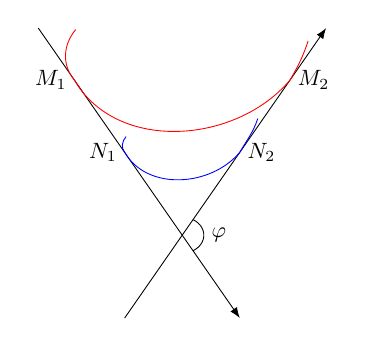
\begin{tikzpicture}[scale=0.8]
  \begin{axis}[clip=false,xmin=-3, xmax=3,ymin=-3,ymax=3, grid=none,
    xtick=\empty, ytick=\empty, axis lines=none, smooth]

    % y = 1.732 * x
    % y = -1.732 * x
    \draw [-Latex] (-0.8,-1.386) -- (2,3.464);
    \draw [-Latex] (-2,3.464) -- (0.8,-1.386);

    % -------------------------------------------------
    % 辅助线
    % \addplot[draw=blue,domain=-2.5:-0.5] {1.732 * x + 6};
    % \addplot[draw=blue,domain=0.5:2.5] {3 * x - 2};

    % 曲线 M1M2
    \draw [red] (-1.48,3.44) to [out=-130,in=130] (-1.5,2.598);
    \draw [red] (-1.5,2.598) to [out=-60,in=-130] (1.5,2.598);
    \draw [red] (1.5,2.598) to [out=60,in=-108.43] (1.75,3.25);

    % -------------------------------------------------
    % 辅助线
    % \addplot[draw=red,domain=-1.5:0] {1.732 * x + 3};
    % \addplot[draw=red,domain=0:1.5] {3 * x - 1.2};

    % 曲线 N1N2
    \draw [blue] (-0.78,1.65) to [out=-130,in=130] (-0.8,1.386);
    \draw [blue] (-0.8,1.386) to [out=-60,in=-130] (0.8,1.386);
    \draw [blue] (0.8,1.386) to [out=60,in=-108.43] (1.05,1.95);

    \node [left] at (-1.5,2.598) {$M_1$};
    \node [right] at (1.5,2.5988) {$M_2$};
    \node [left] at (-0.8,1.386) {$N_1$};
    \node [right] at (0.8,1.386) {$N_2$};

    % 倾角
    \draw [domain=-60:60] plot ({0.3*cos(\x)}, {0.3*sin(\x)});
    \node [right] at (0.3,0) {$\varphi$};

  \end{axis}
\end{tikzpicture}

      \subcaption{角度$\varphi$相同,长度不同}
      \label{curvature_exam2}
  \end{subfigure}
  \caption{曲线弧的弯曲程度}
  \label{曲线弧的弯曲程度}
\end{figure}

\subsubsection{曲率概念}
\paragraph{}
设曲线$C$是光滑的,在曲线$C$上选定一点$M_0$作为度量弧$s$的基点。设曲线上点$M$对应于弧$s$,在点$M$处切线的倾角为$\alpha$,曲线上另外一点$M'$对应于弧$s+\Delta s$,在点$M'$处切线的倾角为$\alpha+\Delta\alpha$,那么弧段$\overarc{MM'}$的长度为$|\Delta s|$,当动点从$M$移动到$M'$时切线转过的角度为$|\Delta\alpha|$。

\paragraph{}
我们用比值$\displaystyle \big|\frac{\Delta\alpha}{\Delta s}\big|$,即单位弧段上切线转过的角度的大小来表达弧段$\overarc{MM'}$的平均弯曲程度,把这比值叫做弧段$\overarc{MM'}$的\uwave{平均曲率},并记作$\overline{K}$,即

\begin{equation}
  \overline{K} = \big|\frac{\Delta\alpha}{\Delta s}\big|.
\end{equation}

\begin{figure}[H]
\centering
  % 曲率概念
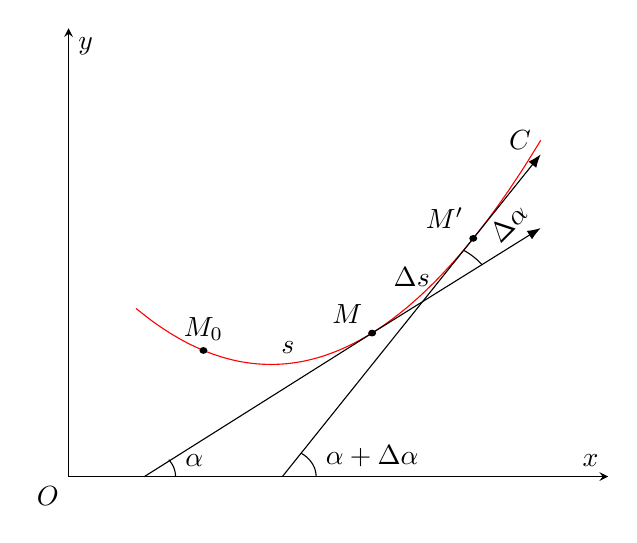
\begin{tikzpicture}[scale=1]
  \begin{axis}[clip=false,xmin=0, xmax=8,ymin=0,ymax=8, grid=none,
    xtick=\empty, ytick=\empty, axis lines=middle,
    smooth, xlabel={$x$}, ylabel={$y$}]

    % 曲线 C
    % y' = 0.5*(x-3)
    \addplot[draw=red,domain=1:7] {(x-3)^2/4 + 2};

    % 弧段
    \node [above] at (3.25,2.02) {$s$};
    \node [left] at (5.5,3.56) {$\Delta s$};

    % 切线
    % y = 0.75 * x - 0.815
    \draw [-Latex] (1.125,0) -- (4.5,2.56) -- (7,4.434);
    % y = 1.5 * x - 4.75
    \draw [-Latex] (3.17,0) -- (6,4.25) -- (7,5.75);

    % 标记
    \node [left] at (7,6) {$C$};
    \node [above] at (2,2.25) {$M_0$};
    \draw [fill] (2,2.25) circle [radius=0.05];
    \node [above left] at (4.5,2.56) {$M$};
    \draw [fill] (4.5,2.56) circle [radius=0.05];
    \node [above left] at (6,4.25) {$M'$};
    \draw [fill] (6,4.25) circle [radius=0.05];

    % 倾角
    \draw [domain=0:36.88] plot ({1.086 + 0.5*cos(\x)}, {0.5*sin(\x)});
    \node [above right] at (1.586,0) {$\alpha$};

    \draw [domain=0:56.6] plot ({3.17 + 0.5*cos(\x)}, {0.5*sin(\x)});
    \node [above right] at (3.67,0) {$\alpha + \Delta\alpha$};

    \draw [domain=36.88:56.6] plot ({5.25 + 1.1 * cos(\x)}, {3.12 + 1.1 * sin(\x)});
    \node [above right,rotate=45] at (6.4,3.9) {$\Delta\alpha$};

    % 原点
    \node [below left] at (0,0) {$O$};
  \end{axis}
\end{tikzpicture}

  \caption{曲率概念}
  \label{曲率概念}
\end{figure}

\paragraph{}
类似于从平均速度引进瞬时速度的方法,当$\Delta s \to 0$时(即$M' \to M$时),上述平均曲率的极限叫做曲线$C$在点$M$处的\uwave{曲率},记作$K$,即

\begin{equation}
  K = \lim_{\Delta s \to 0}\big|\frac{\Delta\alpha}{\Delta s}\big|.
\end{equation}

在$\displaystyle\lim_{\Delta s \to 0}\frac{\Delta\alpha}{\Delta s}=\frac{d\alpha}{ds}$存在的条件下,$K$也可以表示为
\begin{equation}
  \label{曲率的定义式}
  K = \big|\frac{d\alpha}{ds}\big|.
\end{equation}

\paragraph{}
直线的切线与本身重合,切线的倾角$\alpha$不变,曲率为$K=0$。半径为$a$的圆,其曲率为$\displaystyle K=\frac{1}{a}$。

\subsubsection{直角坐标方程的曲率计算推导}
\paragraph{}
在一般情况下,我们根据\eqref{曲率的定义式}式来导出便于实际计算曲率的公式。
\paragraph{}
设曲线的直角坐标方程是$y=f(x)$,且$f(x)$具有二阶导数(这时$f'(x)$连续,从而曲线是光滑的)。因为$\tan\alpha=y'$,所以

\begin{align}
\begin{split}
  y'' =&\; (y')' \\
      =&\; (\tan\alpha)' \quad \text{(复合函数求导法则)} \\
      =&\; \sec^2\alpha \bigcdot (\alpha)' \\
     =&\; \sec^2\alpha \bigcdot \frac{\Delta\alpha}{\Delta x},
\end{split}
\end{align}
又因为
\begin{equation}
  \tan^2\alpha + 1 = \sec^2\alpha,
\end{equation}
所以
\begin{equation}
  \frac{d\alpha}{dx} = \frac{y''}{1+\tan^2\alpha}=\frac{y''}{1+y'^2},
\end{equation}
于是
\begin{equation}
  d\alpha=\frac{y''}{1+y'^2}dx.
\end{equation}
又由\eqref{弧微分公式}知道
\begin{equation}
  ds = \sqrt{1+y'^2}dx.
\end{equation}
从而,根据曲率$K$的表达式\eqref{曲率的定义式},有
\begin{equation}
  \label{直角坐标方程的曲率计算公式}
  K = \frac{|y''|}{(1+y'^2)^{3/2}}.
\end{equation}

\subsubsection{参数方程的曲率计算推导}
\paragraph{}
设曲线由参数方程
\begin{equation}
  \left\{\begin{array}{l}
    x=\varphi(t), \\
    y=\psi(t)
  \end{array} \right.
\end{equation}
给出,则可利用由参数方程所确定的函数的求导法,求出$y'_x$及$y''_x$,代入\eqref{直角坐标方程的曲率计算公式}便得

\begin{equation}
  K=\frac{|\varphi'(t)\psi''(t)-\varphi''(t)\psi'(t)|}{[\varphi'^2(t)+\psi'^2(t)]^{3/2}}.
\end{equation}

\subsection{曲率圆与曲率半径}
\paragraph{}
设曲线$y=f(x)$在点$M(x,y)$处的曲率为$K(k\neq0)$。在点$M$处的曲线的法线上,在凹的一侧取一点$D$,使$\displaystyle|DM|=\frac{1}{K}=\rho$。以$D$为圆心,$\rho$为半径作圆,这个圆叫做曲线在点$M$处的\uwave{曲率圆},曲率圆的圆心$D$叫做曲线在点$M$处的\uwave{曲率中心},曲率圆的半径$\rho$叫做曲线在点$M$处的\uwave{曲率半径}。

\begin{figure}[H]
\centering
  % 曲率圆
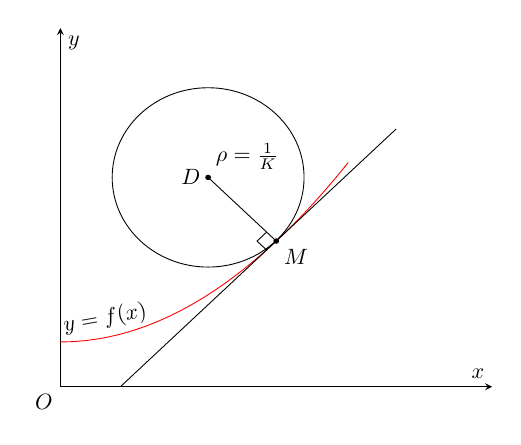
\begin{tikzpicture}[scale=0.8]
  \begin{axis}[clip=false,xmin=0, xmax=9,ymin=0,ymax=8, grid=none,
    xtick=\empty, ytick=\empty, axis lines=middle,
    smooth, xlabel={$x$}, ylabel={$y$}]

    % 曲线 y=f(x)
    % y' = 0.222 * x
    % y'' = 0.222
    \addplot[draw=red,domain=0:6] {x^2/9 + 1};

    % 弧段
    \node [above,rotate=10] at (1,1.11) {$y=f(x)$};
    \draw [fill] (4.5,3.25) circle [radius=0.05];
    \node [below right] at (4.5,3.25) {$M$};

    % 切线
    % y = x - 1.25
    \draw (1.25,0) -- (4.5,3.25) -- (7,5.75);

    % 曲率:K = 0.222 / (1+y'^2)^3/2 --> x = 4.5 --> K = 0.079
    % 半径:p = 1 / K = 12.73
    % 法线:y = -x + 7.75

    \draw [fill] (3.08,4.67) circle [radius=0.05];
    \draw (3.08,4.67) -- (4.5,3.25);
    \draw (3.08,4.67) circle [radius=2];
    \node [left] at (3.08,4.67) {$D$};
    \node [above right] at (3.08,4.67) {$\rho=\frac{1}{K}$};

    % y = -x + 7.35
    % y = x - 0.85
    \draw (4.3,3.05) -- (4.1,3.25) -- (4.3,3.45);

    % 原点
    \node [below left] at (0,0) {$O$};
  \end{axis}
\end{tikzpicture}

  \caption{曲率圆}
  \label{曲率圆}
\end{figure}

\paragraph{}
常常用曲率圆在点$M$邻近的一段圆弧来近似代替曲线弧,使问题简化。

\paragraph{}
按上述规定,曲线在点$M$处的曲率$K(k\neq0)$与曲线在点$M$处的曲率半径$\rho$有如下关系:
\begin{equation}
  \rho=\frac{1}{K}, \; K = \frac{1}{\rho}.
\end{equation}

  \section{方程的近似解}
    \subsection{方程的近似解}
\paragraph{}
求解高次代数方程或其它类型的方程的问题。求得这类方程的实根的精确值,比较困难,因此,可以寻求方程的近似解。

\begin{enumerate}
  \item 确定根的大致范围,确定一个区间$[a,b]$,使所求的根位于这区间内。这一步工作称为\uwave{根的隔离},区间$[a,b]$称为所求实根的\uwave{隔离区间}。
  \item 以根的隔离区间的端点作为根的初始近似值,逐步逼近精确值,或在精确度范围内的值。
\end{enumerate}

\subsubsection{二分法}
\paragraph{}
设$f(x)$在区间$[a,b]$上连续,$f(a)\bigcdot f(b) < 0$,且方程$f(x)=0$在$(a,b)$内仅有一个实根$\xi$,于是$[a,b]$即是这个根的一个隔离区间。

\paragraph{}
取$[a,b]$的中点$\displaystyle \xi_1 = \frac{a+b}{2}$,计算$f(\xi_1)$,然后不断缩小隔离区间的范围,不断计算中点$\xi_1$直到$f(\xi_1)=0$或在精确度之内$f(\xi_1) - 0 < \varepsilon$

\subsubsection{切线法}
\paragraph{}
用曲线弧一端的切线来代替曲线弧,从而求出方程实根的近似值。这种方法叫做\uwave{切线法}。端点的选取根据下面$4$种情况。
\begin{figure}[H]
\centering
  %------- 第1行 -------
  \begin{subfigure}[t]{0.45\linewidth}
    \centering
      % 切线法的 4 种不同情形
\begin{tikzpicture}[scale=0.8]
  \begin{axis}[clip=false,xmin=0, xmax=8,ymin=-4,ymax=4, grid=none,
    xtick=\empty, ytick=\empty, axis lines=middle,
    smooth, xlabel={$x$}, ylabel={$y$}]

    % y' = 0.15*(x-1)^0.5*x + 0.1 * (x-1)^1.5
    \addplot[draw=red,domain=1:5.5] {0.1 * (x-1)^1.5 * x - 2};

    % 实根
    \node [above] at (3.95,0) {$\xi$};

    % A
    \draw [dashed] (1,-2) -- (1,0);
    \draw [fill] (1,-2) circle [radius=0.05];
    \node [left] at (1,-2) {$A$};
    \node [above] at (1,0) {$a$};

    % B
    \draw [dashed] (5.5,3.25) -- (5.5,0);
    \draw [fill] (5.5,3.25) circle [radius=0.05];
    \node [right] at (5.5,3.25) {$B$};
    \node [below] at (5.5,0) {$b$};

    \node [below left] at (5,3.25) {$y=f(x)$};

    % 切线
    \addplot[domain=4.3:5.5] {2.7*x - 11.6};
    \node [below] at (4.3,0) {$x_1$};

    % 原点
    \node [left] at (0,0) {$O$};
  \end{axis}
\end{tikzpicture}

      \subcaption{$f(a)<0,f(b)>0$\newline$f'(x)>0,f''(x)>0$}
  \end{subfigure}
  \begin{subfigure}[t]{0.45\linewidth}
    \centering
      % 切线法的 4 种不同情形
\begin{tikzpicture}[scale=0.8]
  \begin{axis}[clip=false,xmin=0, xmax=8,ymin=-4,ymax=4, grid=none,
    xtick=\empty, ytick=\empty, axis lines=middle,
    smooth, xlabel={$x$}, ylabel={$y$}]

    % y' = -20*(x+1)^-2
    \addplot[draw=red,domain=1.5:6] {20/(x+1) - 5};

    % 实根
    \node [above] at (3,0) {$\xi$};

    % A
    \draw [dashed] (1.5,3) -- (1.5,0);
    \draw [fill] (1.5,3) circle [radius=0.05];
    \node [left] at (1.5,3) {$A$};
    \node [below] at (1.5,0) {$a$};

    \node [below right] at (1.8,3) {$y=f(x)$};

    % 切线
    \addplot[domain=1.5:2.44] {-3.2*x + 7.8};
    \node [below] at (2.44,0) {$x_1$};

    % B
    \draw [dashed] (6,-2.14) -- (6,0);
    \draw [fill] (6,-2.14) circle [radius=0.05];
    \node [right] at (6,-2.14) {$B$};
    \node [above] at (6,0) {$b$};

    % 原点
    \node [left] at (0,0) {$O$};
  \end{axis}
\end{tikzpicture}

      \subcaption{$f(a)>0,f(b)<0$\newline$f'(x)<0,f''(x)>0$}
  \end{subfigure}
  %------- 第2行 -------
  \begin{subfigure}[t]{0.45\linewidth}
    \centering
      % 切线法的 4 种不同情形
\begin{tikzpicture}[scale=0.8]
  \begin{axis}[clip=false,xmin=0, xmax=8,ymin=-4,ymax=4, grid=none,
    xtick=\empty, ytick=\empty, axis lines=middle,
    smooth, xlabel={$x$}, ylabel={$y$}]

    % y' = 3/x
    \addplot[draw=red,domain=1.5:6] {3*ln(x) - 3.5};

    % 实根
    \node [below] at (3.23,0) {$\xi$};

    % A
    \draw [dashed] (1.5,-2.28) -- (1.5,0);
    \draw [fill] (1.5,-2.28) circle [radius=0.05];
    \node [left] at (1.5,-2.28) {$A$};
    \node [above] at (1.5,0) {$a$};

    % 切线
    \addplot[domain=1.5:2.64] {2*x - 5.28};
    \node [above] at (2.64,0) {$x_1$};

    % B
    \draw [dashed] (6,1.88) -- (6,0);
    \draw [fill] (6,1.88) circle [radius=0.05];
    \node [right] at (6,1.88) {$B$};
    \node [below] at (6,0) {$b$};

    \node [below left] at (5,1.88) {$y=f(x)$};

    % 原点
    \node [left] at (0,0) {$O$};
  \end{axis}
\end{tikzpicture}

      \subcaption{$f(a)<0,f(b)>0$\newline$f'(x)>0,f''(x)<0$}
  \end{subfigure}
  \begin{subfigure}[t]{0.45\linewidth}
    \centering
      % 切线法的 4 种不同情形
\begin{tikzpicture}[scale=0.8]
  \begin{axis}[clip=false,xmin=0, xmax=8,ymin=-4,ymax=4, grid=none,
    xtick=\empty, ytick=\empty, axis lines=middle,
    smooth, xlabel={$x$}, ylabel={$y$}]

    % -0.6*(x-1)^0.8
    \addplot[draw=red,domain=1:6] {-0.33*(x-1)^1.8+2.5};

    % 实根
    \node [below left] at (4.248,0) {$\xi$};

    % A
    \draw [dashed] (1,2.5) -- (1,0);
    \draw [fill] (1,2.5) circle [radius=0.05];
    \node [left] at (1,2.5) {$A$};
    \node [below] at (1,0) {$a$};

    \node [below right] at (2.5,2.5) {$y=f(x)$};

    % B
    \draw [dashed] (6,-3.48) -- (6,0);
    \draw [fill] (6,-3.48) circle [radius=0.05];
    \node [right] at (6,-3.48) {$B$};
    \node [above] at (6,0) {$b$};

    % 切线
    \addplot[domain=4.41:6] {-2.17*x + 9.57};
    \node [above] at (4.41,0) {$x_1$};

    % 原点
    \node [left] at (0,0) {$O$};
  \end{axis}
\end{tikzpicture}

      \subcaption{$f(a)>0,f(b)<0$\newline$f'(x)<0,f''(x)<0$}
  \end{subfigure}

  \caption{切线的$4$种不同情形}
  \label{切线的4种不同情形}
\end{figure}

\paragraph{}
假设选取端点为$a$的情形,令$x_0 = a$,在端点$(x_0,f(x_0))$作切线,这切线的方程为
\begin{equation*}
  y - f(x_0) = f'(x_0)(x-x_0)
\end{equation*}
令$y=0$,可以解出$x_1$为
\begin{equation*}
  x_1 = x_0 - \frac{f(x_0)}{f'(x_0)}
\end{equation*}

\paragraph{}
然后继续在点$(x_1,f(x_1))$作切线,直到逼近$\xi$,一般的,在点$(x_{n-1},f(x_{n-1}))$作切线,得根的近似值
\begin{equation}
  x_n = x_{n-1} - \frac{f(x_{n-1})}{f'(x_{n-1})}.
\end{equation}


  \newpage
  \part{不定积分}
  \section{不定积分的概念与性质}
    \subsection{原函数与不定积分的概念}
\paragraph{}
\textbf{定义1\;}如果在区间$I$上,可导函数$F(x)$的导函数为$f(x)$,即对任一$x\in I$,都有
\begin{equation}
  F'(x) = f(x) \;\textbf{或}\; dF(x) = f(x)dx,
\end{equation}
那么函数$F(x)$就称为$f(x)$(或$f(x)dx$)在区间$I$上的\uwave{原函数}。

\paragraph{}
\textbf{原函数存在定理\;}如果函数$f(x)$在区间$I$上连续,那么在区间$I$上存在可导函数$F(x)$,使对任一$x\in I$都有
\begin{equation*}
  F'(x) = f(x).
\end{equation*}
即\textbf{连续函数一定有原函数}。

\paragraph{}
\textbf{定义2\;}在区间$I$上,函数$f(x)$的带有任意常数项的原函数称为$f(x)$(或$f(x)dx$)在区间$I$上的\uwave{不定积分},记作
\begin{equation}
  \int{f(x)dx},
\end{equation}
其中记号$\int$称为\uwave{积分号},$f(x)$称为\uwave{被积函数},$f(x)dx$称为\uwave{被积表达式},$x$称为\uwave{积分变量}。

\paragraph{}
由此定义及前面的说明可知,如果$F(x)$是$f(x)$在区间$I$上的一个原函数,那么$F(x)+C$就是$f(x)$的不定积分,即
\begin{equation}
  \int{f(x)dx} = F(x) + C.
\end{equation}
因而不定积分$\int{f(x)dx}$可以表示$f(x)$的任意一个原函数。

\subsection{基本积分表}
\paragraph{}

\bgroup
\def\arraystretch{3}
\setlength\tabcolsep{0.8cm}
\begin{table}[H]
\centering
  \caption{基本积分表}
  \begin{tabular}{l|l}
    \hline
    $\displaystyle\int{kdx}=kx+C(k\text{是常数})$ &
    $\displaystyle\int{x^\mu dx}=\frac{x^{\mu+1}}{\mu+1} + C(\mu \neq -1)$ \\
    \hline
    $\displaystyle\int{\frac{dx}{x}} = \ln{|x|} + C$ &
    $\displaystyle\int{\frac{dx}{1+x^2}} = \arctan{x} + C$ \\
    \hline
    $\displaystyle\int{\frac{dx}{\sqrt{1-x^2}}} = \arcsin{x} + C$ &
    $\displaystyle\int{\cos{x}dx} = \sin{x} + C$ \\
    \hline
    $\displaystyle\int{\sin{x}dx} = -\cos{x} + C$ &
    $\displaystyle\int{\frac{dx}{\cos^2x}} = \int{\sec^2xdx} = \tan{x} + C$ \\
    \hline
    $\displaystyle\int{\frac{dx}{\sin^2x}} = \int{\csc^2xdx} = -\cot{x} + C$ &
    $\displaystyle\int{\sec{x}\tan{x}dx} = \sec{x} + C$ \\
    \hline
    $\displaystyle\int{\csc{x}\cot{x}dx} = -\csc{x} + C$ &
    $\displaystyle\int{e^xdx} = e^x + C$ \\
    \hline
    $\displaystyle\int{a^xdx} = \frac{a^x}{\ln{a}} + C$ & \\
    \hline
  \end{tabular}
\end{table}
\egroup

\subsection{不定积分的性质}
\paragraph{}
\textbf{性质1\;}设函数$f(x)$及$g(x)$的原函数存在,则
\begin{equation}
  \int{[f(x)+g(x)]dx} = \int{f(x)dx} + \int{g(x)}dx.
\end{equation}

\paragraph{}
\textbf{性质2\;}设函数$f(x)$的原函数存在,$k$为非零常数,则
\begin{equation}
  \int{kf(x)dx}=k\int{f(x)dx}.
\end{equation}

  \section{换元积分法}
    \subsection{第一类换元法}
\paragraph{}
设$f(u)$具有原函数$F(u)$,即
\begin{equation}
  F'(u) = f(u), \; \int{f(u)du} = F(u) + C.
\end{equation}
如果$u$是中间变量:$u=\varphi(x)$,且设$\varphi(x)$可微,那么,根据复合函数微分法,有
\begin{equation}
  dF[\varphi(x)] = f[\varphi(x)]\varphi'(x)dx,
\end{equation}
从而根据不定积分的定义就得
\begin{equation}
 \int f[\varphi(x)]\varphi'dx=F[\varphi(x)] + C = \big[\int f(u)du\big]_{u=\varphi(x)}.
\end{equation}
因此:

\paragraph{}
\textbf{定理\;}设$f(u)$具有原函数,$u=\varphi(x)$可导,则有\textbf{换元公式}
\begin{equation}
  \int f[\varphi(x)]\varphi'(x)dx = \big[\int f(u)du\big]_{u=\varphi(x)}.
\end{equation}

\subsubsection{例子1}
\paragraph{}
被积函数中含有三角函数,需要用到一些三角恒等式。

\paragraph{}
\textbf{例子1\;}求$\displaystyle\int{\sin^3xdx}$

\paragraph{}
\textbf{解\;}三角恒等变换后,令$u=\cos{x}$作变换。
\begin{align*}
\begin{split}
  \int\sin^3xdx \;=&\; \int\sin^2x\sin{x}dx \\
  =&\; -\int(1-\cos^2x)d(\cos{x}) \\
  =&\; -\cos{x} + \frac{1}{3}\cos^3{x} + C.
\end{split}
\end{align*}

\subsubsection{例子2}
\paragraph{}
对于$\sin^{2k+1}x\cos^nx$或$\sin^nx\cos^{2k+1}x$(其中$k\in N$)型函数的积分,总可依次作变换$u=\cos{x}$或$u=\sin{x}$,求得结果。

\paragraph{}
\textbf{例子2\;}求$\displaystyle\int{\sin^2x\cos^5xdx}$

\paragraph{}
\textbf{解\;}三角恒等变换后,令$u=\sin{x}$作变换。
\begin{align*}
\begin{split}
  \int\sin^2x\cos^5xdx \;=&\; \int\sin^2x\cos^4x\cos{x}dx \\
    =&\; \int\sin^2x(1-\sin^2x)^2d(\sin{x})  \\
    =&\; \int(\sin^2x-2\sin^4x + \sin^6x)d(\sin{x}) \\
    =&\; \frac{1}{3}\sin^3x-\frac{2}{5}\sin^5x+\frac{1}{7}\sin^7x + C.
\end{split}
\end{align*}

\subsubsection{例子3}
\label{第一类换元法例子3}
\paragraph{}
对于$\sin^{2k}x\cos^{2t}x \; (k,l \in N)$型的函数,总可利用三角恒等式:$\displaystyle\sin^2x=\frac{1}{2}(1-\cos{2x}),$ \\ $ \cos^2x = \frac{1}{2}(1+\cos{2x})$化成$\cos{2x}$的多项式。

\paragraph{}
\textbf{例子3\;}求$\displaystyle\int\sin^2x\cos^4xdx$

\paragraph{}
\textbf{解\;}三角恒等变换化简后,对多项式进行求积分
\begin{align*}
\begin{split}
  \int\sin^2x\cos^4xdx \;=&\; \frac{1}{8}\int(1-\cos{2x})(1+\cos{2x})^2dx \\
  =&\; \frac{1}{8} \int (1+\cos{2x} - \cos^2{2x} - \cos^3{2x})dx \\
  =&\; \frac{1}{8} \int (\cos{2x} - \cos^3{2x})dx + \frac{1}{8} \int (1 - \cos^2{2x})dx \\
  =&\; \frac{1}{8} \int \cos{2x}(1 - \cos^2{2x})dx + \frac{1}{8} \int (1 - \cos^2{2x})dx \\
  =&\; \frac{1}{8} \int \sin^2{2x} \bigcdot \frac{1}{2}d(\sin{2x}) + \frac{1}{8} \int \frac{1}{2} (1-\cos{4x}dx) \\
  =&\; \frac{1}{48} \sin^3{2x} + \frac{x}{16} - \frac{1}{64} \sin{4x} + C.
\end{split}
\end{align*}

\subsubsection{例子4}
\paragraph{}
对于$\tan^nx\sec^{2k}x$或$\tan^{2k-1}x\sec^nx \; (k \in N^+)$型函数的积分,可依次变换$u=\tan{x}$或$u=\sec{x}$,求得结果。

\paragraph{}
\textbf{例子4\;}求$\displaystyle\int\tan^5x\sec^3xdx$

\paragraph{}
\textbf{解\;}利用$\tan^2x = \sec^2x-1; \; (\sec{x})' = \sec{x}\tan{x}$
\begin{align*}
\begin{split}
  \int\tan^5x\sec^3xdx \;=&\; \int\tan^4x\sec^2x\sec{x}\tan{x}dx \\
  =&\; \int(\sec^2x-1)^2\sec^2xd(\sec{x}) \\
  =&\; \int(\sec^6x-2\sec^4x+\sec^2x)d(\sec{x}) \\
  =&\; \frac{1}{7}\sec^7x - \frac{2}{5}\sec^5x + \frac{1}{3}\sec^3x + C
\end{split}
\end{align*}

\subsection{第二类换元法}
\paragraph{}
第一类换元法是通过变量代换\uwave{$u=\varphi(x)$},将积分$\displaystyle\int{f[\varphi(x)]\varphi'(x)dx}$化为积分$\displaystyle\int{f(u)du}$.

\paragraph{}
第二类换元法是:选择适当的变量代换\uwave{$x=\psi(t)$},将积分$\displaystyle\int{f(x)dx}$化为积分 \\ $\displaystyle\int{f[\psi(t)]\psi'(t)dt}$。与第一类换元法的区别是,变量代换不同,公式和思路方向相反。

\paragraph{}
\textbf{定理2\;}设$x=\psi(t)$是单调的、可导的函数,并且$\psi'(t)\neq 0$,又设$f[\psi(t)]\psi'(t)$具有原函数,则有换元公式
\begin{equation}
  \int f(x)dx = \big[\int f[\psi(t)]\psi'(t)dt\big]_{t=\psi^-1(x)},
\end{equation}
其中$\psi^{-1}(x)$是$x=\psi(t)$的反函数。

\subsubsection{例子1}
\paragraph{}
有根式$\sqrt{a^2 - x^2}$,可以利用三角公式$\sin^2t+\cos^2t=1$来化去根式。

\paragraph{}
\textbf{例子1\;}求$\displaystyle \int\sqrt{a^2 - x^2}dx \; (a > 0)$。

\paragraph{}
\textbf{解\;}设$x=a\sin{t}, \; -\frac{\pi}{2} < t < \frac{\pi}{2}$,那么$\sqrt{a^2-x^2}=\sqrt{a^2-a^2\sin^2t} = a\cos{t}, dx = a\cos{t}dt$,于是根式化成了三角式,所求积分化为
\begin{equation}
  \int\sqrt{a^2-x^2}dx = \int a\cos{t} \bigcdot a\cos{t}dt = a^2\int \cos^2tdt.
\end{equation}
利用第一类换元法\linkref[第一类换元法例子3]{例子3}里的方法,得到
\begin{align*}
\begin{split}
  \int\sqrt{a^2 - x^2}dx \;=&\; a^2(\frac{t}{2}+\frac{\sin{2t}}{4}) + C \\
  =&\; \frac{a^2}{2}t + \frac{a^2}{2}\sin{t}\cos{t} + C.
\end{split}
\end{align*}
由于$x=a\sin{t},\; -\frac{\pi}{2} < t < \frac{\pi}{2}$,所以
\begin{align*}
  t \;=&\; \arcsin\frac{x}{a} \\
  \cos{t} = \sqrt{1-\sin^2t} \;=&\; \sqrt{1-(\frac{x}{a})^2} = \frac{\sqrt{a^2-x^2}}{a},
\end{align*}
于是所求积分为
\begin{equation*}
  \int\sqrt{a^2-x^2}dx = \frac{a^2}{2}\arcsin\frac{x}{a} + \frac{1}{2}x\sqrt{a^2-x^2} + C.
\end{equation*}

\subsubsection{例子2}
\paragraph{}
有根式$\sqrt{a^2 + x^2}$,可以利用三角公式$1 + \tan^2t = \sec^2t$来化去根式。

\subsubsection{例子3}
\paragraph{}
有根式$\sqrt{x^2 - a^2}$,可以利用三角公式$\sec^2t - 1 = \tan^2t$来化去根式。

\subsubsection{例子4}
\paragraph{}
上面的根式$\sqrt{x^2 \pm a^2}$,也可利用公式$\ch^2t - \sh^2t = 1$,采用代换$x=a\sh{t}$或$x=\pm a\ch{t}$来化去根式。

\paragraph{}
新增双曲函数积分公式:
\begin{enumerate}
  \item $\displaystyle\int\sh{x}dx = \ch{x} + C$,
  \item $\displaystyle\int\ch{x}dx = \sh{x} + C$。
\end{enumerate}

\subsection{倒代换}
\paragraph{}
利用倒代换,可消去被积函数的分母中的变量因子$x$。

\paragraph{}
\textbf{例子\;}求$\displaystyle\int\frac{\sqrt{a^2-x^2}}{x^4}dx$。

\paragraph{}
\textbf{解\;}设$\displaystyle x=\frac{1}{t}$,那么$\displaystyle dx = -\frac{dt}{t^2}$,于是
\begin{align*}
\begin{split}
  \int\frac{\sqrt{a^2-x^2}}{x^4}dx \;=&\; \int\frac{\sqrt{a^2-\frac{1}{t^2}} \bigcdot (-\frac{dt}{t^2})}{\frac{1}{t^4}} \\
  =&\; -\int(a^2t^2-1)^{\frac{1}{2}}|t|dt,
\end{split}
\end{align*}
当$x>0$时,有
\begin{align*}
\begin{split}
  \int\frac{\sqrt{a^2-x^2}}{x^4}dx \;=&\; -\frac{1}{2a^2}\int(a^2t^2-1)^{\frac{1}{2}}d(a^2t^2-1) \\
  =&\; -\frac{(a^2t^2-1)^{\frac{3}{2}}}{3a^2} + C \\
  =&\; -\frac{(a^2-x^2)^{\frac{3}{2}}}{3a^2x^3} + C,
\end{split}
\end{align*}
当$x<0$时,有相同的结果。

  \section{分部积分法}
    \subsection{分部积分法}
\paragraph{}
设函数$u=u(x)$及$v=v(x)$具有连续导数。那么,两个函数乘积的导数公式为
\begin{equation}
  (uv)' = u'v + uv',
\end{equation}
移项,得
\begin{equation}
  uv' = (uv)' - u'v.
\end{equation}
对这个等式两边求不定积分,得
\begin{equation}
  \label{分部积分公式}
  \int uv'dx = uv - \int u'vdx.
\end{equation}
公式\eqref{分部积分公式}称为\uwave{分部积分公式}。如果求$\displaystyle \int uv'dx$有困难,而求$\displaystyle \int u'vdx$比较容易时,分部积分公式就可以发挥作用了。

\paragraph{}
为简便起见,也可把公式\eqref{分部积分公式}写成下面的形式:
\begin{equation}
  \int udv = uv - \int vdu.
\end{equation}

\subsection{技巧}
\paragraph{}
选取$u$和$dv$一般要考虑下面两点:
\begin{enumerate}
  \item $v$要容易求得;
  \item $\displaystyle \int vdu$要比$\displaystyle \int udv$容易积出。
\end{enumerate}

\paragraph{}
如果被积函数是幂函数与正(余)弦函数或幂函数与指数函数的乘积,就可以考虑设幂函数为$u$。这样用一次分部积分法就可以使幂函数的幂次降低一次。这里假定幂指数是正整数。

\paragraph{}
\textbf{例子1\;}求$\displaystyle\int x^2e^xdx$

\paragraph{}
\textbf{解\;}设$u=x^2, dv = e^xdx = d(e^x)$,那么
\begin{equation*}
  \int x^2e^xdx = \int x^2d(e^x) = x^2e^x - \int e^xd(x^2) = x^2e^x - 2\int xe^xdx.
\end{equation*}
这样就将$x$的幂次降低了一次。对$\displaystyle\int xe^xdx$再使用一次分部积分法就可以了。于是:
\begin{align*}
\begin{split}
  \int x^2e^xdx \;=&\; \int x^2d(e^x) = x^2e^x - \int e^xd(x^2) = x^2e^x - 2\int xe^xdx. \\
  =&\; x^2e^x - 2(xe^x-e^x) + C \\
  =&\; e^x(x^2-2x+2)+C.
\end{split}
\end{align*}

\paragraph{}
如果被积函数是幂函数与对数函数或幂函数与反三角函数的乘积,就可以考虑设对数函数或反三角函数为$u$。

\paragraph{}
\textbf{例子2\;}求$\displaystyle\int x\arctan{x}dx$

\paragraph{}
\textbf{解\;}用到$\displaystyle (\arctan{x})' = \frac{1}{1+x^2}$
\begin{align*}
\begin{split}
  \int x\arctan{x}dx \;=&\; \frac{1}{2}\int \arctan{x}d(x^2) \\
  =&\; \frac{x^2}{2}\arctan{x} - \frac{1}{2}\int \frac{x^2}{1+x^2}dx \\
  =&\; \frac{x^2}{2}\arctan{x} - \frac{1}{2}\int\frac{1+x^2-1}{1+x^2}dx \\
  =&\; \frac{x^2}{2}\arctan{x} - \frac{1}{2}\int(1-\frac{1}{1+x^2})dx \\
  =&\; \frac{x^2}{2}\arctan{x} - \frac{1}{2}\int(x-\arctan{x}) + C \\
  =&\; \frac{1}{2}(x^2+1)\arctan{x} - \frac{1}{2}x + C.
\end{split}
\end{align*}

  \section{有理函数的积分}
    \subsection{有理函数的积分}
\paragraph{}

  \section{积分表的使用}
    \subsection{积分表的使用}
\paragraph{}

\end{document}
